\documentclass[xcolor=pdftex,dvipsnames,table,mathserif,aspectratio=169]{beamer}
\usetheme{metropolis}
%\usetheme{Darmstadt}
%\usepackage{times}
%\usefonttheme{structurebold}

\usepackage[english]{babel}
%\usepackage[table]{xcolor}
\usepackage{pgf,pgfarrows,pgfnodes,pgfautomata,pgfheaps}
\usepackage{amsmath,amssymb,setspace}
\usepackage[latin1]{inputenc}
\usepackage[T1]{fontenc}
\usepackage{relsize}
\usepackage[absolute,overlay]{textpos} 
\newenvironment{reference}[2]{% 
  \begin{textblock*}{\textwidth}(#1,#2) 
      \footnotesize\it\bgroup\color{red!50!black}}{\egroup\end{textblock*}} 

\DeclareMathSizes{10}{10}{6}{6} 


\title [Healthcare and IO]{Willingness to Pay and Healthcare}
\author{C.Conlon }
\institute{Grad IO }
\date{Fall 2019}
\setbeamerfont{equation}{size=\tiny}
\begin{document}

\begin{frame}
\titlepage
\end{frame}


\begin{frame}{Healthcare and IO}
In recent years, IO has made inroads into questions related to healthcare:
\begin{itemize}
\item How do hospital (systems) and insurers interact?
\item What is the value of adding a hospital to an insurer's network?
\item What determines the market power of insurers? hospitals?
\item Can steering incentives (in network/out of network) be effective in reducing costs?
\end{itemize}
\end{frame}

\begin{frame}{Today's Reading:}
In recent years, IO has made inroads into questions related to healthcare:
\begin{itemize}
\item Capps, Dranove, Satterthwaite (2003)
\item Ho AER (2009)
\end{itemize}
\end{frame}



\begin{frame}{CDS(2003): Motivation}
The Government keeps losing hospital mergers (basically all of them):
\begin{itemize}
\item Some people travel enormous distances to get treatment at hospitals (Mayo Clinic, Cleveland Clinic, Johns Hopkins, Mass General, etc.)
\item These cases are lost at the stage of \alert{market definition} under the \alert{hypothetical monopolist test}.
\begin{itemize}
\item Recall: SSNIP of 5\% price increase for all products. If this is not profitable -- include next closest substitute. Continue adding products to define relevant market.
\item Resulting markets are so large (and unconcentrated) that mergers always lead to negligible changes in market power
\end{itemize}
\item What if we could measure relevant markets better?
\end{itemize}
\end{frame} 


\begin{frame}{CDS(2003): Ex-Ante and Ex-Post WTP}
What is the value that $i$ places on having hospital $j$ included in network $G$?
\begin{align*}
U_{i j} &=\alpha R_{j}+H_{j}^{\prime} \Gamma X_{i}+\tau_{1} T_{i j}+\tau_{2} T_{i j} \cdot X_{i}+\tau_{3} T_{i j} \cdot R_{j}-\gamma\left(Y_{i}, Z_{i}\right) P_{j}\left(Z_{i}\right)+\varepsilon_{i j} \\ &=U\left(H_{j}, X_{i}, \lambda_{i}\right)-\gamma\left(X_{i}\right) P_{j}\left(Z_{i}\right)+\varepsilon_{i j} 
\end{align*}

\begin{itemize}
\item $H_{j}=\left[R_{j}, S_{j}\right]$ is partitioned into generic $R$ and diagnosis specific $S$ characteristics.
\item $X_{i}=\left[Y_{i}, Z_{i}\right]$ is partitioned into demographic $Y$ and diagnosis specific $Z$ characteristics.
\item $T_{i j}=T_{j}\left(\lambda_{i}\right)$ distance from $i$'s home to hospital $j$
\item This paper: ignore $\gamma\left(X_{i}\right) P_{j}\left(Z_{i}\right)$ since $P_{j'}(Z_i) \approx P_j(z_i)$
\item Parameters: $[\alpha,\Gamma, \tau]$ and $\gamma(X_i)$.
\end{itemize}
\end{frame} 


\begin{frame}{Deriving WTP}
Assume that $\varepsilon_{ij} \sim$ Type I EV:
\begin{align*}
s_{j}\left(G, X_{i}, \lambda_{i}\right)=\frac{\exp \left[U\left(H_{j}, X_{i}, \lambda_{i}\right)\right]}{\sum_{g \in G} \exp \left[U\left(H_{g}, X_{i}, \lambda_{i}\right)\right]}
\end{align*}
And
\begin{align*}
V^{I U}\left(G, Y_{i}, Z_{i}, \lambda_{i}\right)=E \max _{j \in G}\left[U\left(H_{j}, Y_{i}, Z_{i}, \lambda_{i}\right)+\varepsilon_{i j}\right]=\ln \left[\sum_{j \in G} \exp \left(U\left(H_{j}, Y_{i}, Z_{i}, \lambda_{i}\right)\right)\right]
\end{align*}
\end{frame}

\begin{frame}{Deriving WTP II}
What happens to utility when we remove $j$ from the choice set?
\begin{itemize}
\item \alert{After} you know your diagnosis $Z_i$
\item \alert{Before} you draw your $\varepsilon_{ij}$
\begin{align*}\Delta V_{j}^{I U}\left(G, Y_{i}, Z_{i}, \lambda_{i}\right)  &=V^{I U}\left(G, Y_{i}, Z_{i}, \lambda_{i}\right)-V^{I U}\left(G / j, Y_{i}, Z_{i}, \lambda_{i}\right) \\
&=\left[\frac{1}{1-s_{j}\left(H_{j}, Y_{i}, Z_{i}, \lambda_{i}\right)}\right]
\end{align*}
\end{itemize}
To get dollars we need $\gamma(X_i)$ so that $\Delta W_{ij}^{IU}(G,Y_i,\lambda_i) = \frac{\Delta V_{j}^{I U}\left(G, Y_{i}, Z_{i}, \lambda_{i}\right) }{\gamma(X_i)}$
\end{frame}

\begin{frame}{Ex-Ante WTP}
But at the beginning of the year (when you choose insurance) you don't observe $Z_i$:
\begin{align*}
\ \Delta W_{i j}^{E A}\left(G, Y_{i}, \lambda_{i}\right) &=\int_{Z} \Delta W_{j}^{I U}\left(G, Y_{i}, Z_{i}, \lambda_{i}\right) f\left(Z_{i} | Y_{i}, \lambda_{i}\right) d Z_{i} \\
 &=\int_{Z} \frac{\Delta V_{j}^{I U}\left(G, Y_{i}, Z_{i}, \lambda_{i}\right)}{\gamma\left(Y_{i}, Z_{i},\right)} f\left(Z_{i} | Y_{i}, \lambda_{i}\right) d Z_{i} 
 \end{align*}
 Integrate out (expected) health $Z_i$ conditional on demographics $Y_i$ and location $\lambda_i$.
\begin{align*}
 \Delta W_{j}^{E A}(G) &=N \int_{y, \lambda} \Delta W_{j}^{I U}\left(G, Y_{i}, Z_{i}, \lambda_{i}\right) f\left(Y_{i} | \lambda_{i}\right) d Y_{i} d \lambda_{i} \\ &=N \int_{Y, Z, \lambda} \frac{1}{\gamma\left(Y_{i}, Z_{i}\right)} \ln \left[\frac{1}{1-s_{j}\left(G, Y_{i}, Z_{i}, \lambda_{i}\right)}\right] f\left(Y_{i}, Z_{i}, \lambda_{i}\right) d Y_{i} d Z_{i} d \lambda_{i}
\end{align*}
Aggregate over $N$ consumers and integrate out heterogeneity in the population.
\end{frame}

\begin{frame}{Insurer's Problem}
If the insurer includes hospital $j$ in the network they gain:
\begin{align*}
\pi_{j}=\alpha\left(\Delta W_{j}^{E A}(G)-\Delta C_{j}(G)\right)+u_{j}
\end{align*}
\begin{itemize}
\item $\Delta W_{j}^{E A}(G)$ comes from extra willingness to pay of consumers
\item $\Delta C_{j}(G)$ comes from extra costs (could be negative).
\item $\alpha$ is assumed to be a fixed  constant (share of surplus) $\rightarrow$ \alert{bargaining weight}.
\end{itemize}
\end{frame}

\begin{frame}{In Practice}
In practice CDS have to cut some corners
\begin{itemize}
\item Big problem is that they can't identify $\gamma(X_i)$ and assume $\gamma(X_i) = \gamma_p$.
\begin{itemize}
\item ``True'' model puts most weight on \alert{inelastic} consumers who value income little
\item People who are very sick; people who are very rich.
\end{itemize}
\item They assume $\Delta C_j(G)=0$ so that they can regress
\begin{align*}
\pi_{j}=\frac{\alpha}{\gamma_{P}}\left(\overline{\Delta W}_{j}^{E A}(G)\right)+u_{j}=a\left(\overline{\Delta W}_{j}^{E A}(G)\right)+u_{j}
\end{align*}
\item Probably worry that high quality hospitals are costly ie: $Cov(\xi_j,\omega_j) >0$ in BLP.
\end{itemize}
\end{frame}

\begin{frame}{Data}
\begin{center}
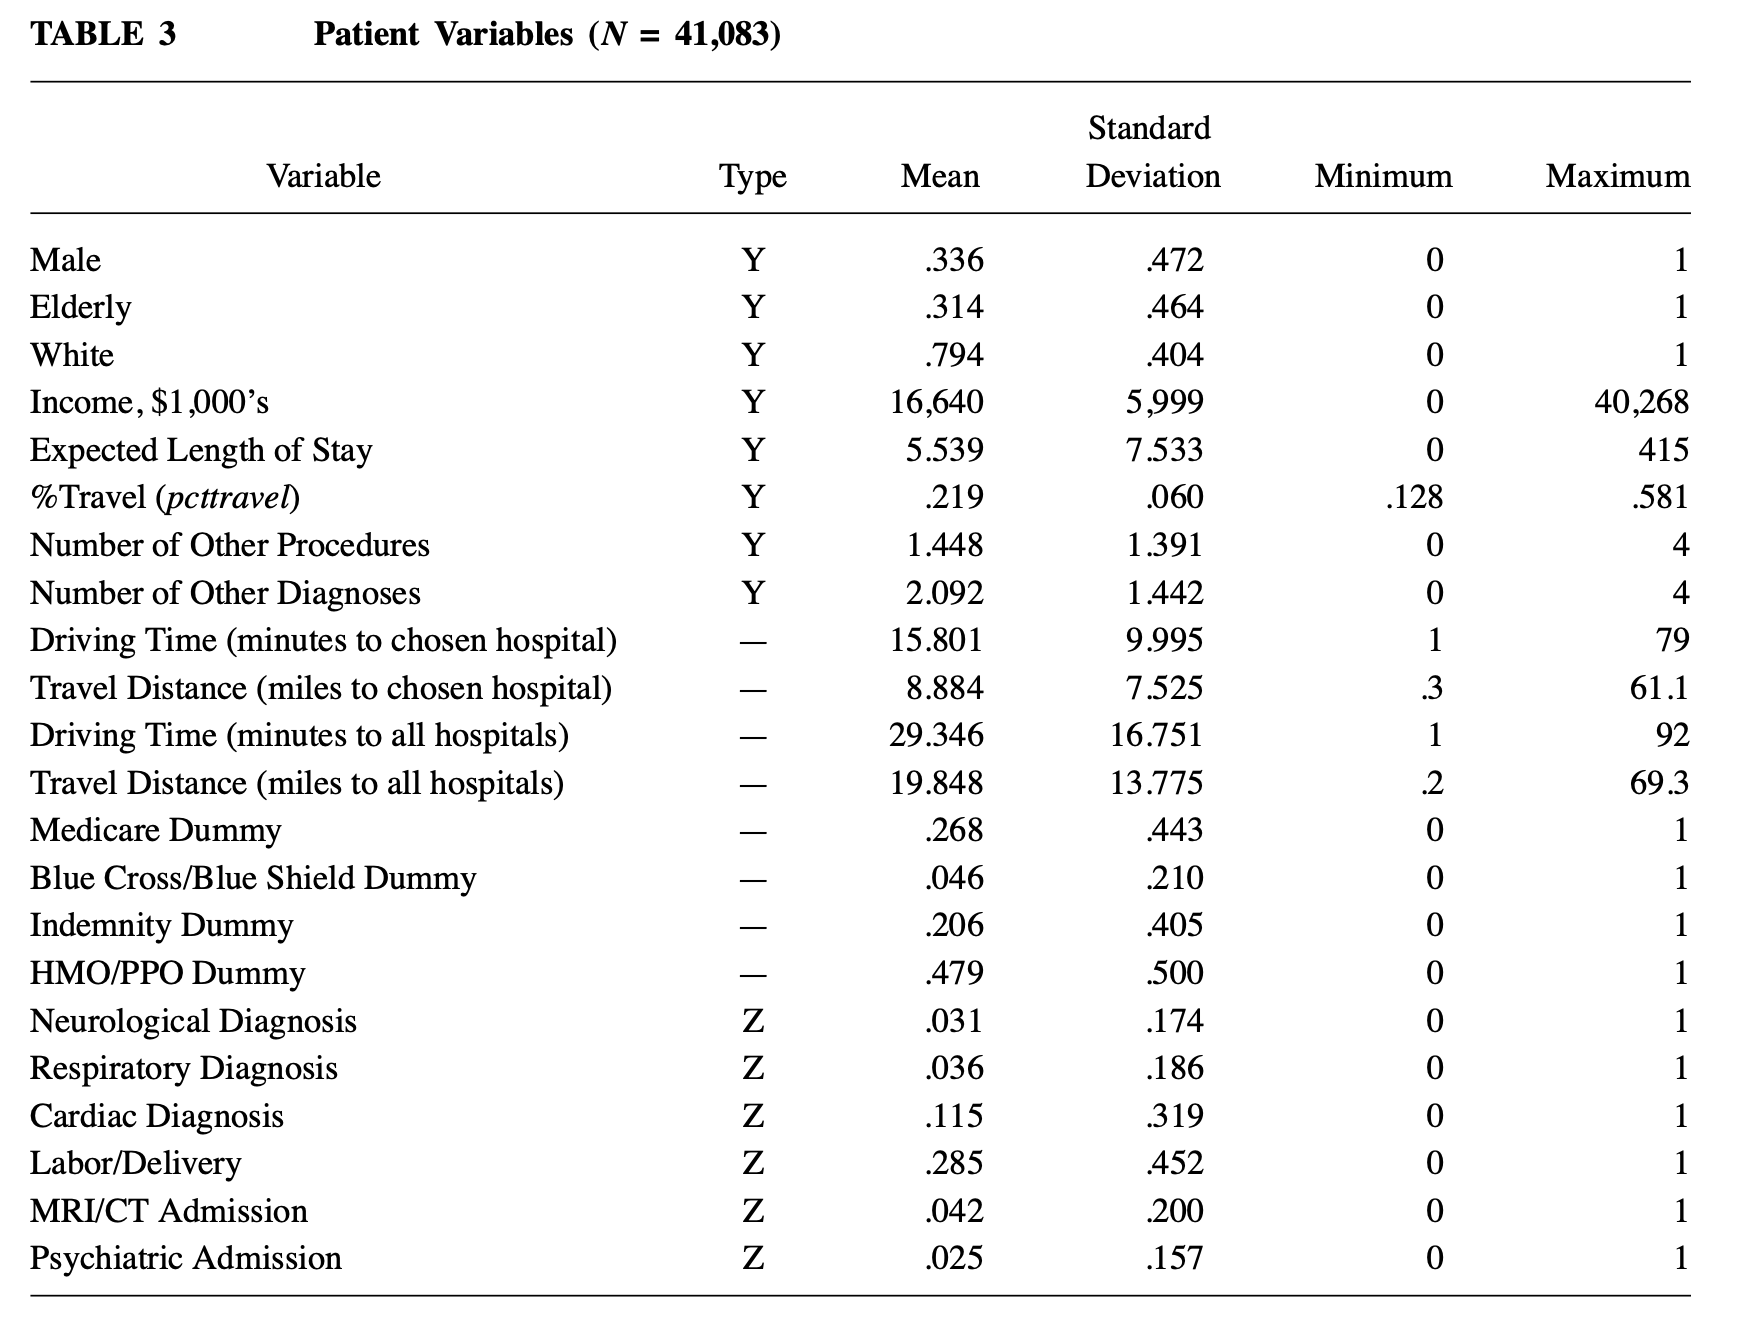
\includegraphics[height=7cm]{./resources/cds_table3.png}
\end{center}
\end{frame}

\begin{frame}{Estimation}
\begin{enumerate}
\item Estimate individual choice logit via MLE (no endogeneity) on different samples (MCO alone, MCO plus indemnity)
\item Estimate the WTP measure $\Delta V_j^{IU}$ (MCO only, MCO+Idemnity) for each hospital.
\item Try to compute cost estimates using admission data.
\item Compute hospital profits using (Revenue - Costs).
\item Regress profits on the WTP measure.
\end{enumerate}
Idea is that high WTP hospitals add more value to network and command more profits.
\end{frame}

\begin{frame}{Do not-for profits exploit market power? (Yes)}
\begin{center}
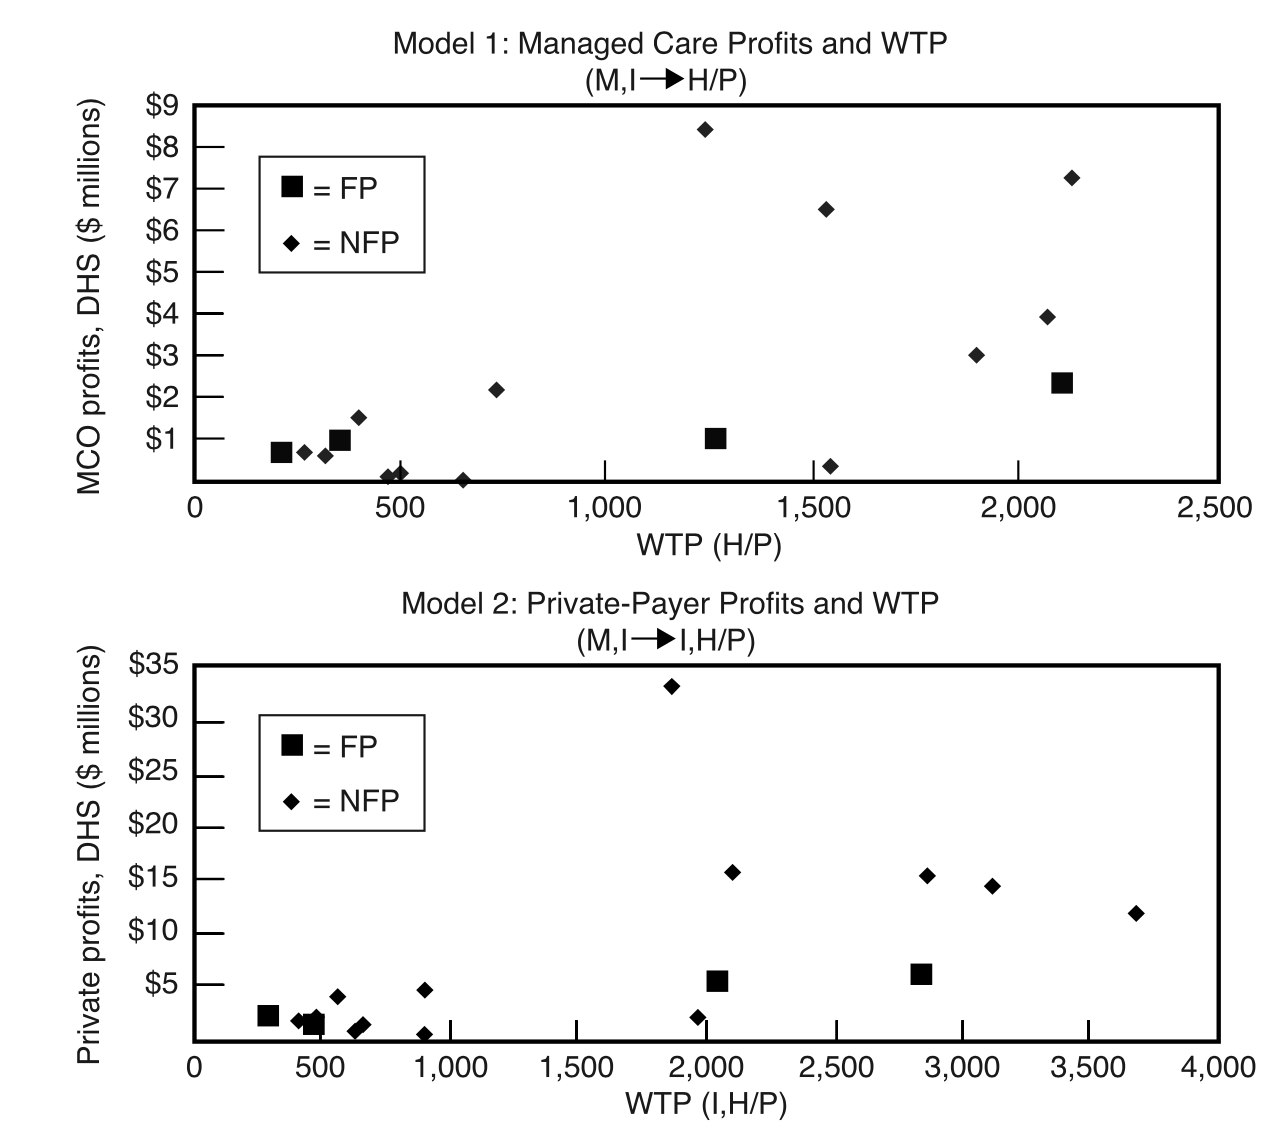
\includegraphics[height=6cm]{./resources/cds_fig1a.png}
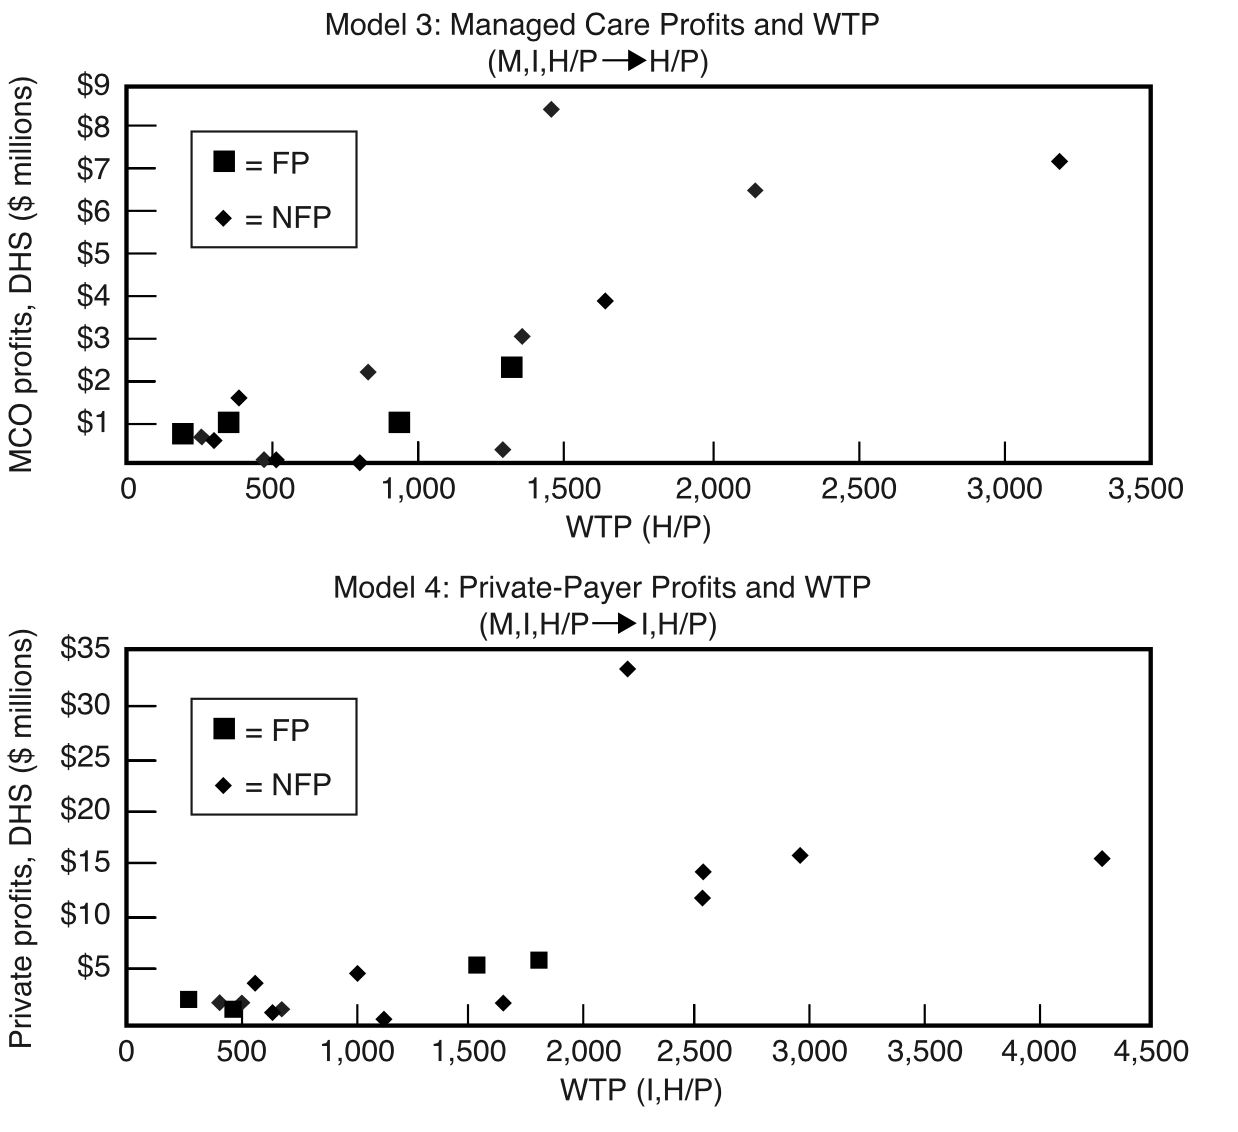
\includegraphics[height=6cm]{./resources/cds_fig1b.png}
\end{center}
\end{frame}


\begin{frame}{Decomposing WTP: UCSD vs. SCV}
\begin{center}
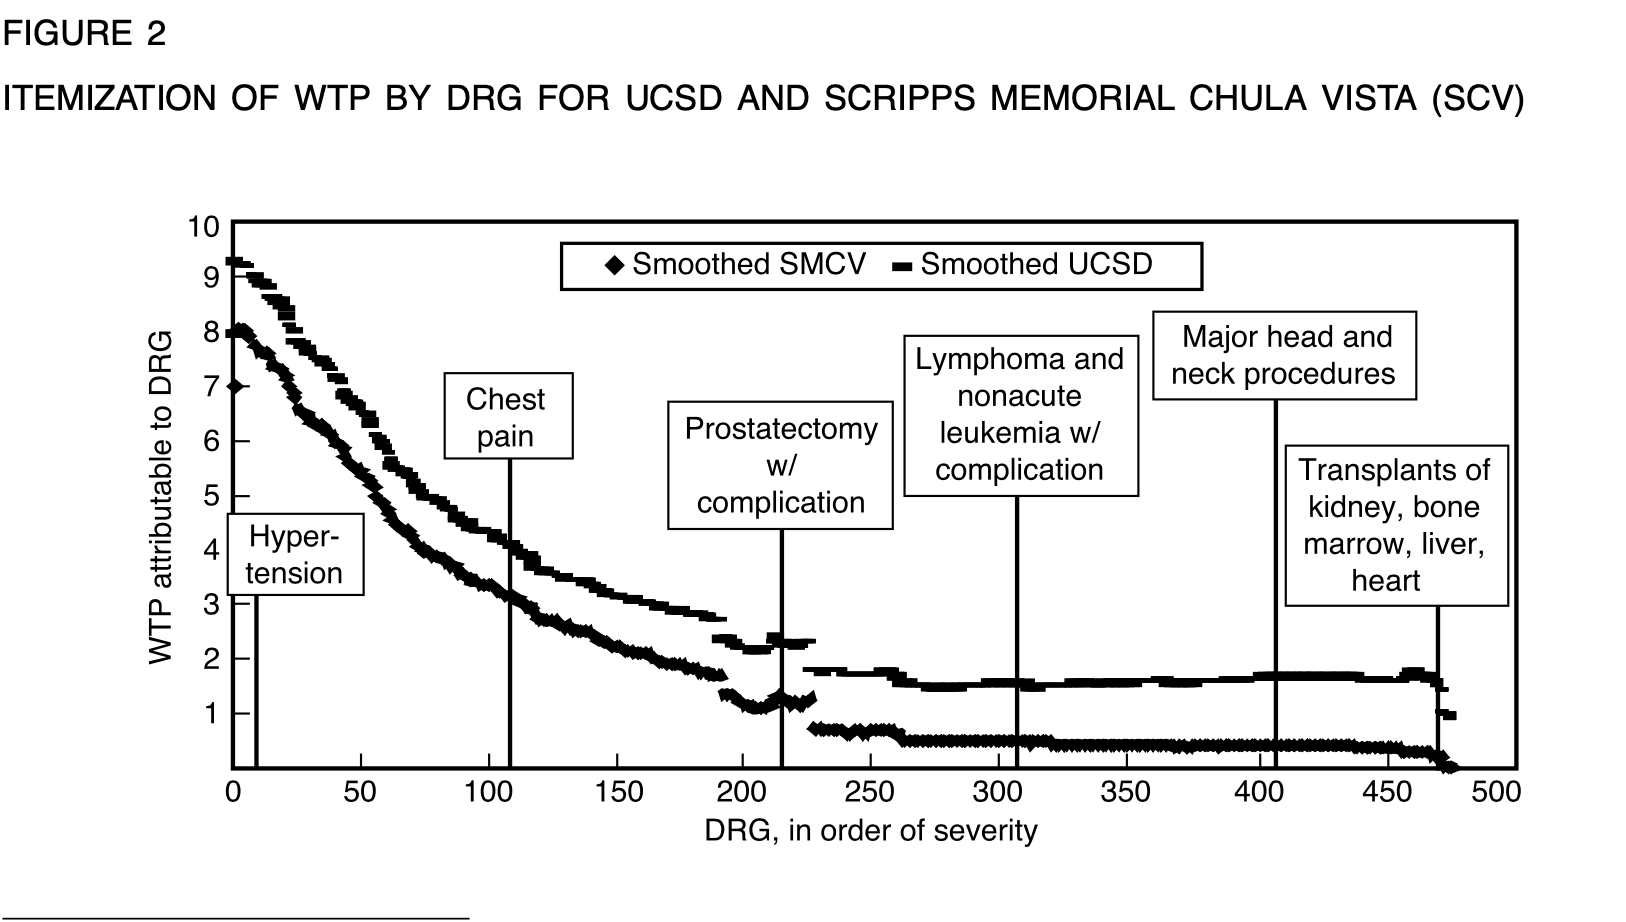
\includegraphics[height=6cm]{./resources/cds_fig2}
\end{center}
UCSD's value is driven by most severe diagnoses.
\end{frame}


\begin{frame}{What might a merger do?}
The merger allows the seller to \alert{bundle} hospitals
\begin{align*}
\overline{\Delta W}_{j+k}^{E A}(G)&=N \int_{Y, Z, \lambda} \ln \left[\frac{1}{1-s_{j}\left(G, Y_{i}, Z_{i}, \lambda_{i}\right)-s_{k}\left(G, Y_{i}, Z_{i}, \lambda_{i}\right)}\right] f\left(Y_{i}, Z_{i}, \lambda_{i}\right) d Y_{i} d Z_{i} d \lambda_{i}\\
\Delta \hat{\pi}_{j+k}&=\hat{a}\left[\overline{\Delta W}_{j+k}^{E A}(G)-\overline{\Delta W}_{j}^{E A}(G)-\overline{\Delta W}_{k}^{E A}(G)\right]
\end{align*}
Where $\hat{a}$ is the coefficient from regression of profits on WTP.
\begin{itemize}
\item Will be largest when products are close substitutes or affect same customers.
\end{itemize}

\end{frame}

\begin{frame}{Case Study: Chula Vista}
\begin{itemize}
\item Three hospitals (Scripps: SCV, Community Hospital: CHCV, Paradise Valley (PVH)
\item Because 30\% of patients leave Chula Vista SSNIP tests tend to say Chula Vista is not its own market.
\item But WTP says otherwise
\end{itemize}
\end{frame}


\begin{frame}{Merger Results}
\begin{center}
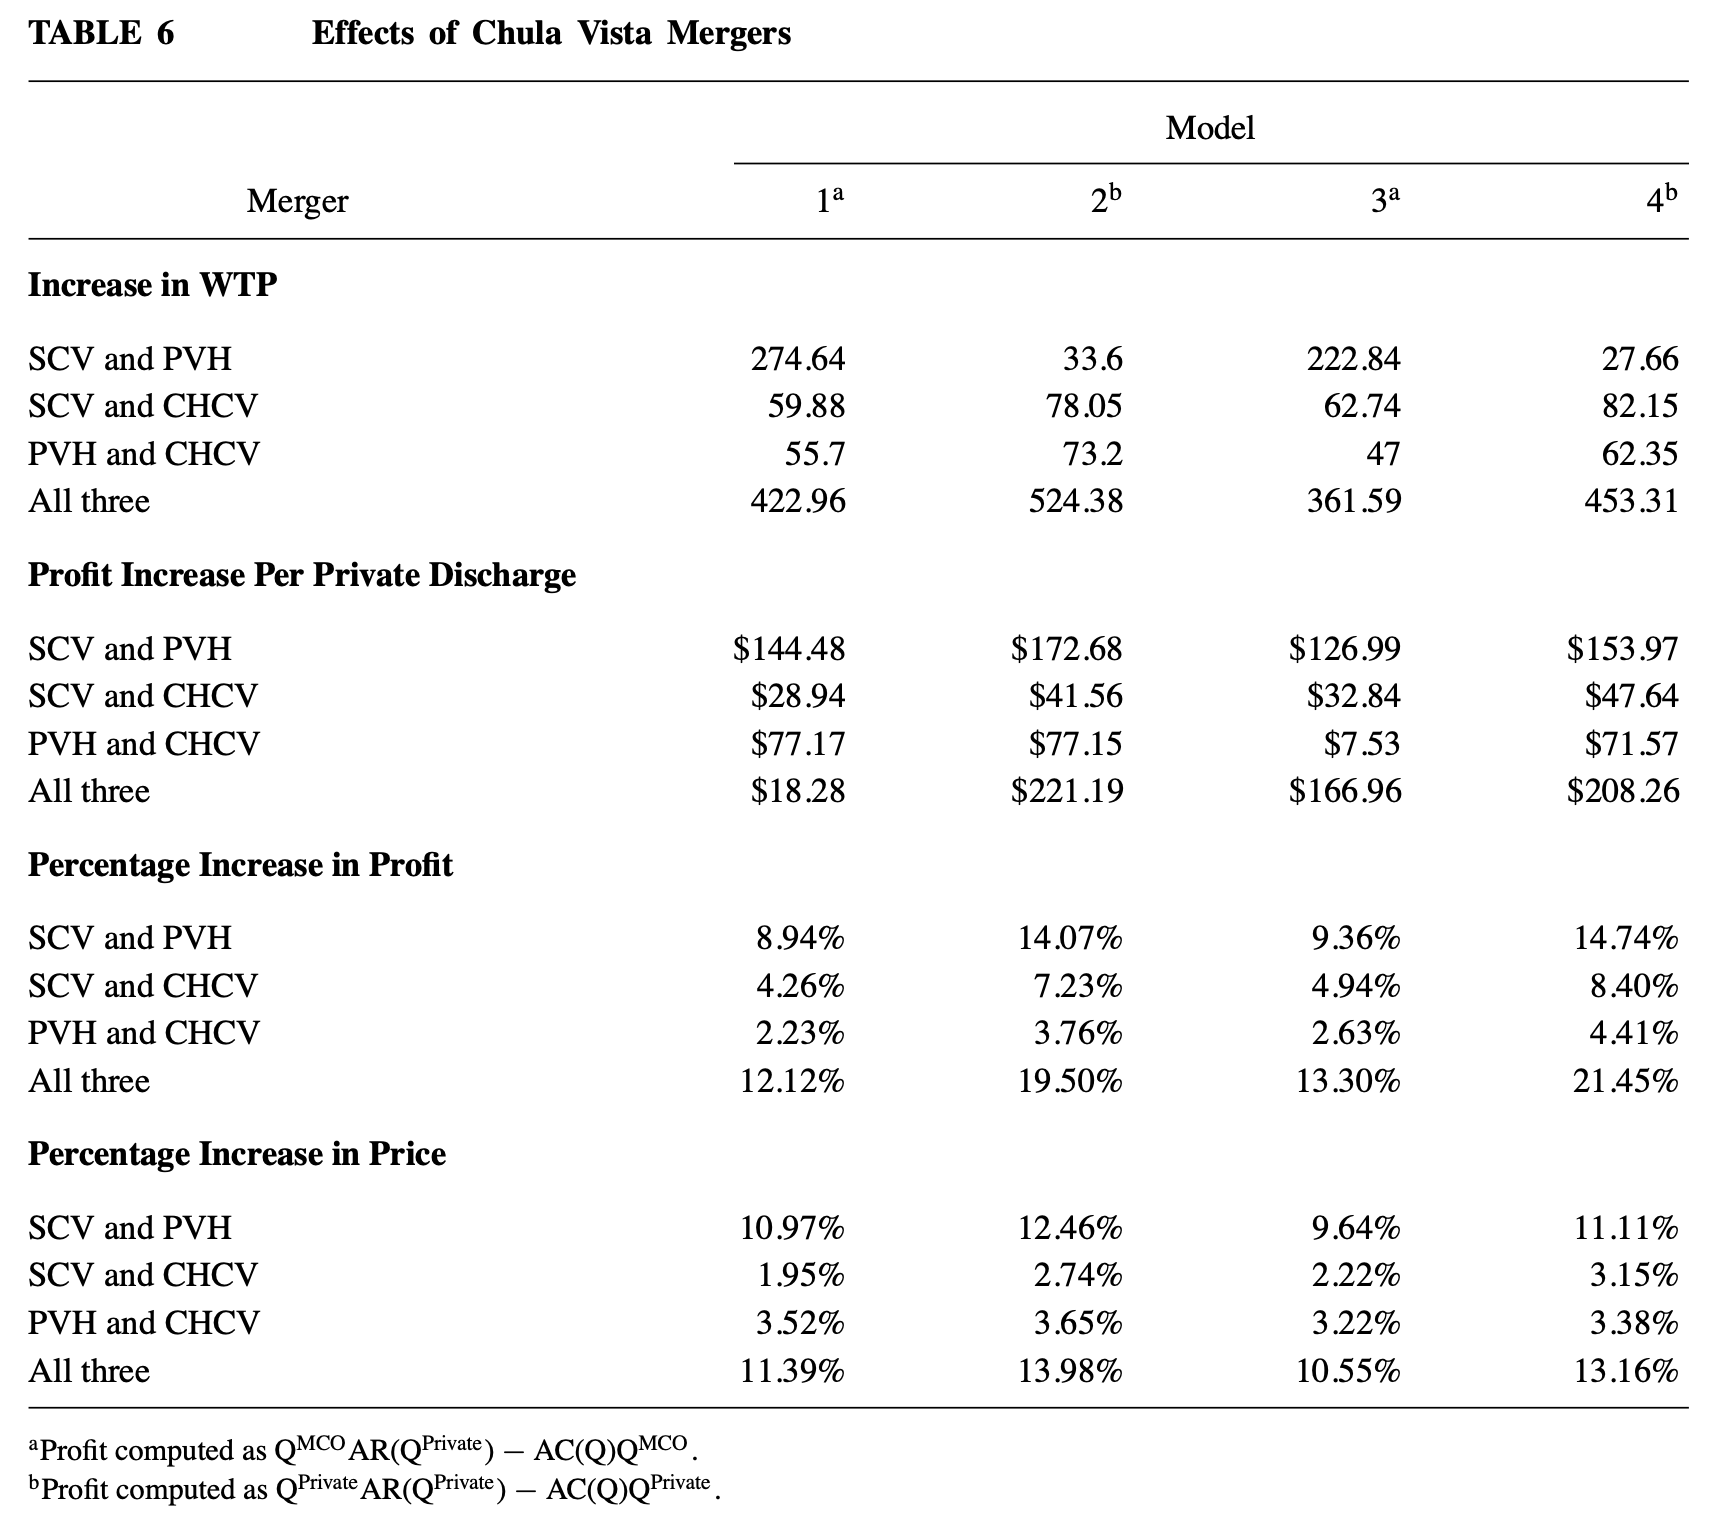
\includegraphics[height=7cm]{./resources/cds_table6.png}
\end{center}
\end{frame}



\begin{frame}{Merger Results}
\begin{center}
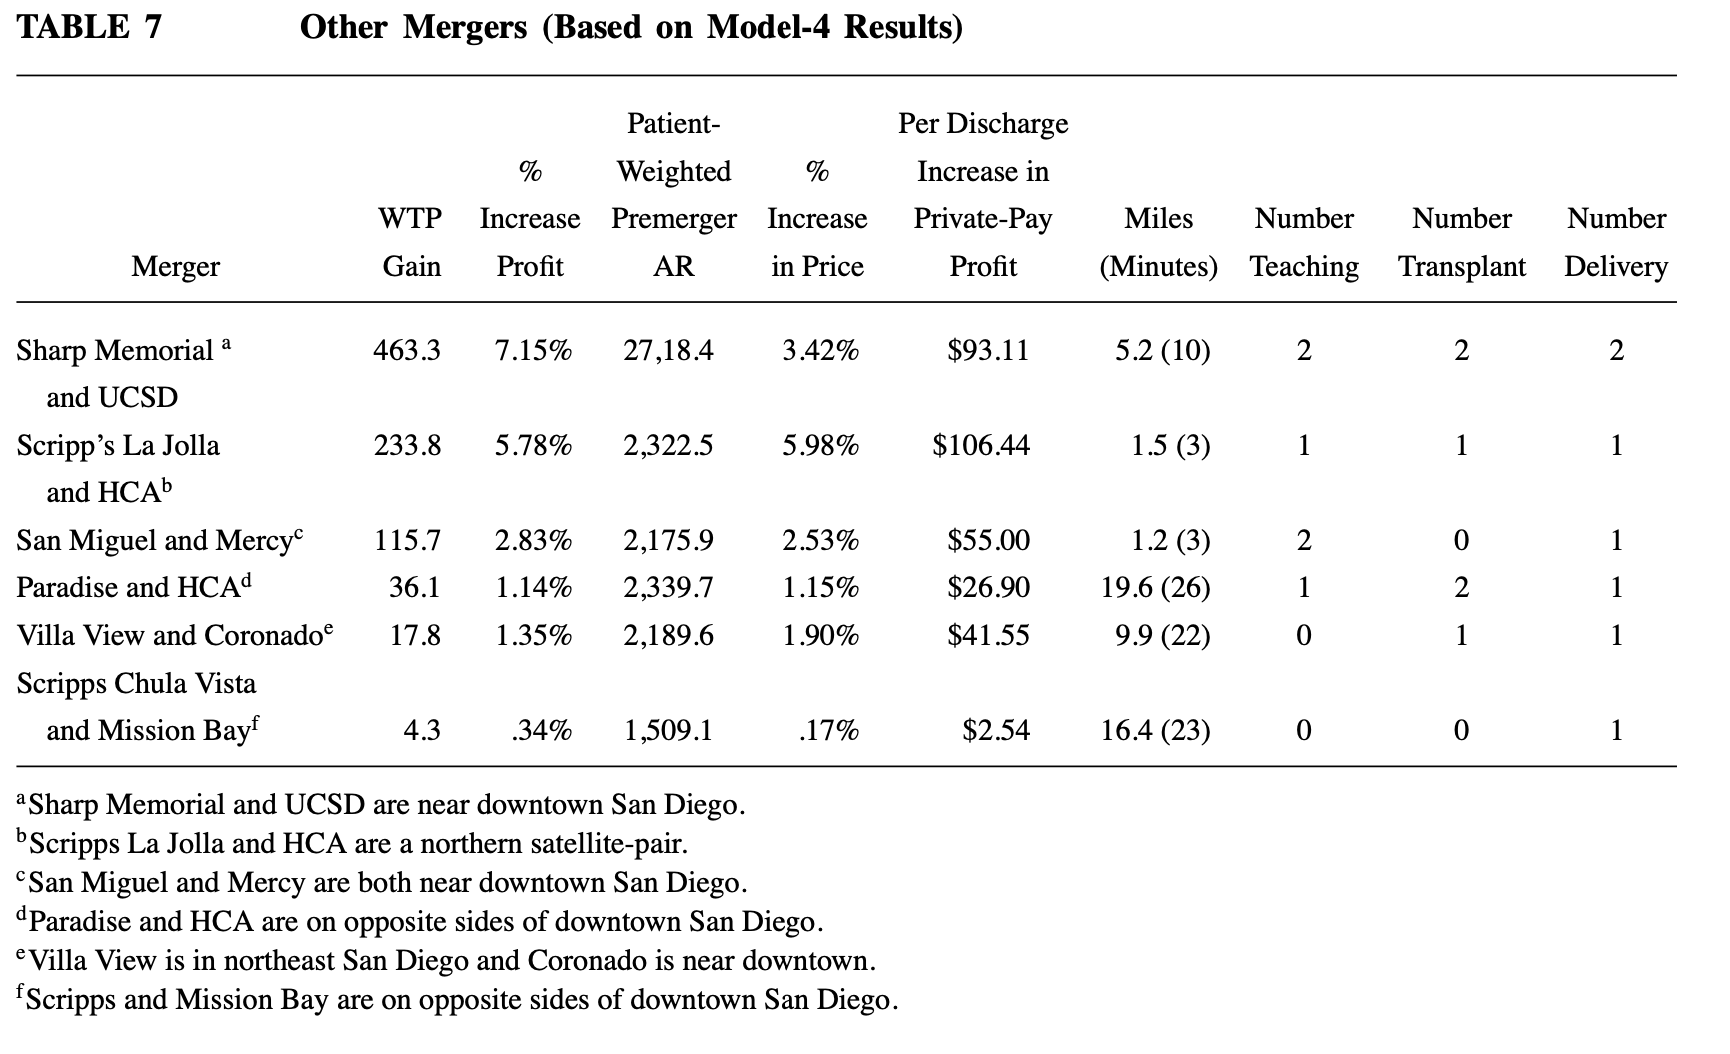
\includegraphics[height=7cm]{./resources/cds_table7.png}
\end{center}
\end{frame}


\section{Ho AER 2009: Insurer-Provider Networks in the Medical Care Market}

\begin{frame}{Research Question}
\begin{itemize}
\item How do insurers and healthcare providers (hospitals) divide profits?
\item How is the division of profits related to the networks of hospitals offered by insurers?
\item Given we know about WTP and \alert{demand}, how can we treat \alert{supply} decisions of endogenous networks and negotiations between firms seriously?
\end{itemize}
\end{frame}

\begin{frame}{Timing of the game}
\begin{enumerate}
\item Hospitals make price offers to plans
\item Plans choose their hospital networks
\item Plans set premiums
\item Consumers and employers jointly choose plans
\item Sick consumers visit hospitals; plans pay hospitals for services provided
\end{enumerate}
Plan choice of quality and products, together with the hospital's choices of capacity, location, services, and quality are outside the model (exogenous).
\end{frame}

\begin{frame}{Hospital Services}
\begin{center}
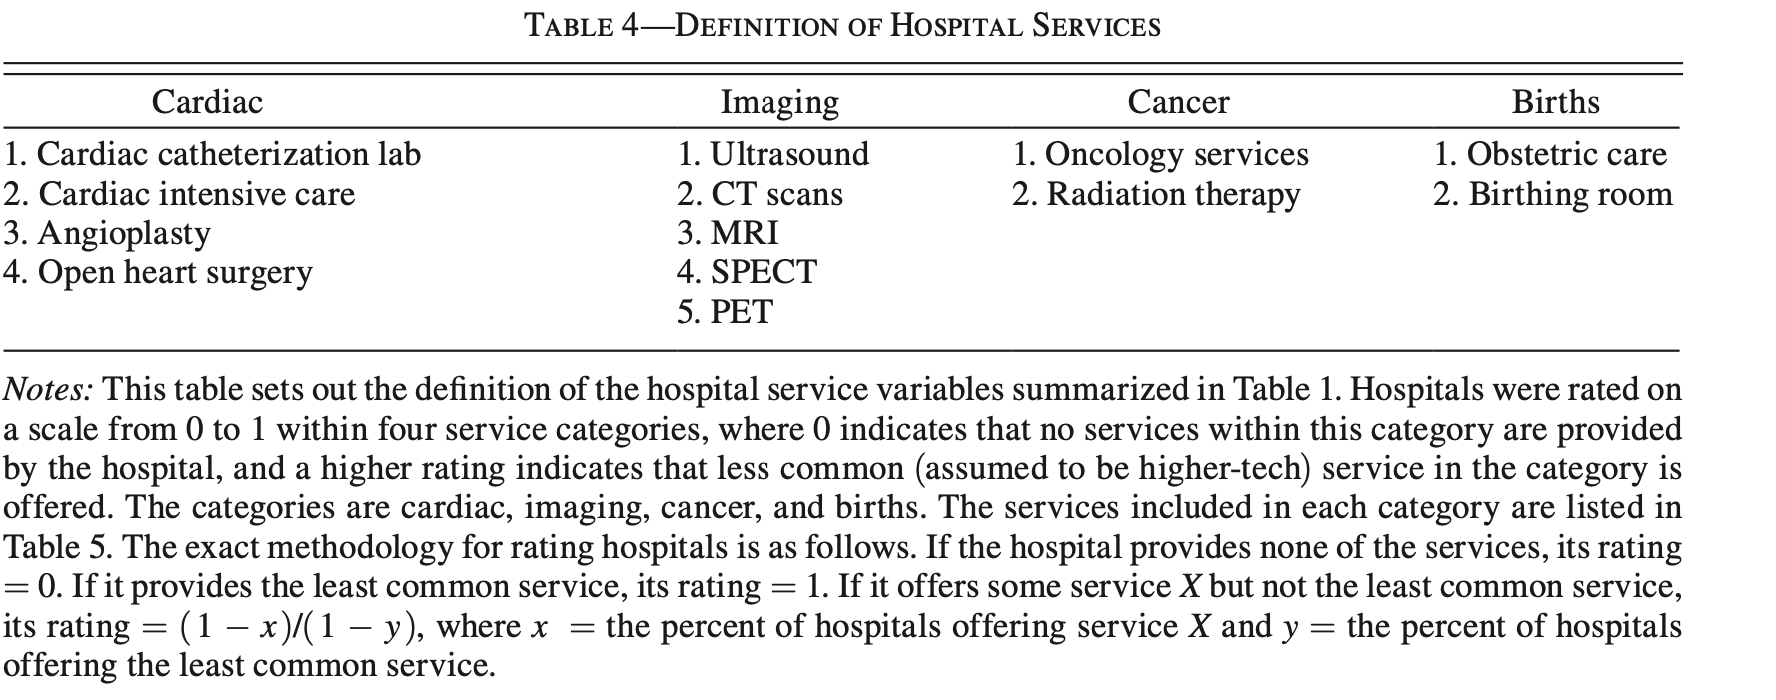
\includegraphics[height=5.5cm]{./resources/ho_table4.png}
\end{center}
Key characteristic: how sophisticated services are for particular diagnoses.
\end{frame}

\begin{frame}{Data: Hospitals}
\begin{center}
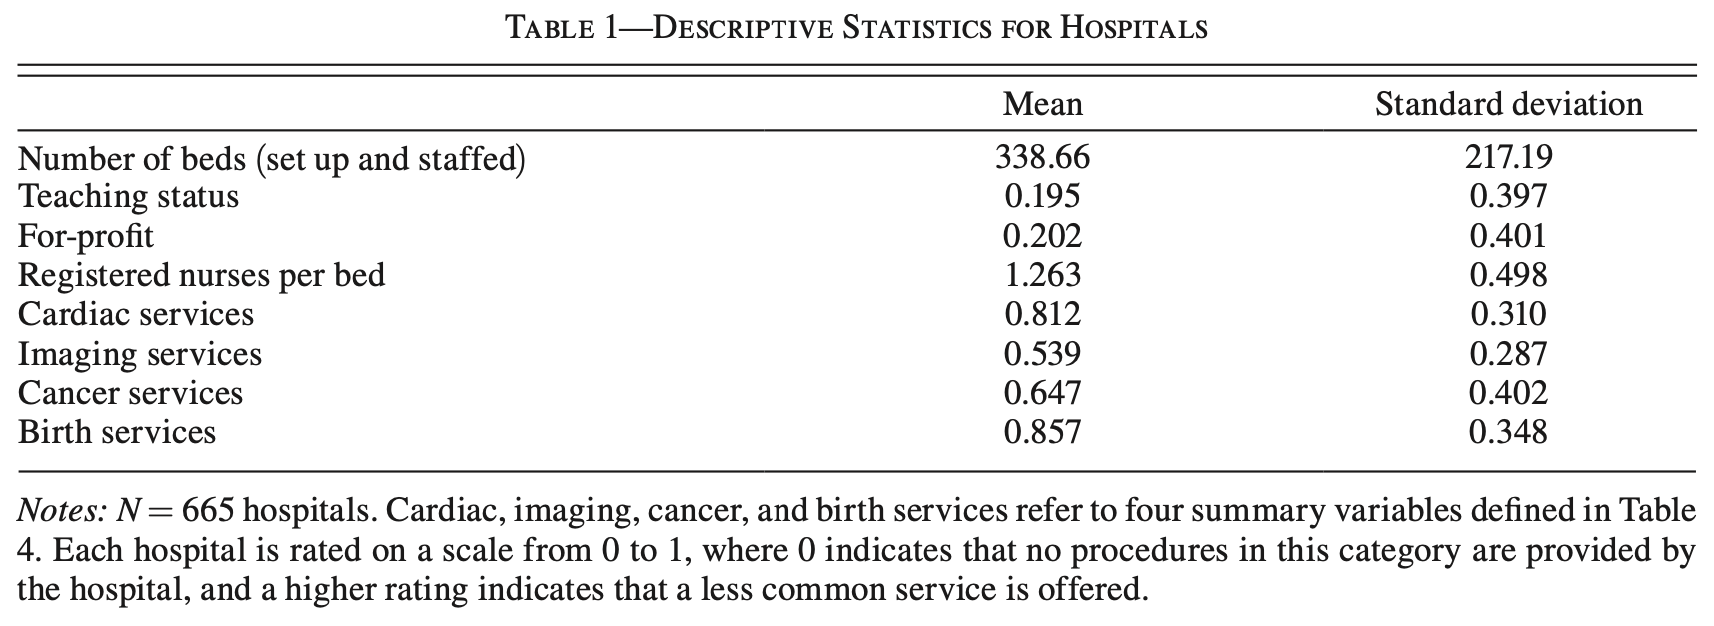
\includegraphics[height=5cm]{./resources/ho_table1.png}
\end{center}
\end{frame}


\begin{frame}{Data: Plans}
\begin{center}
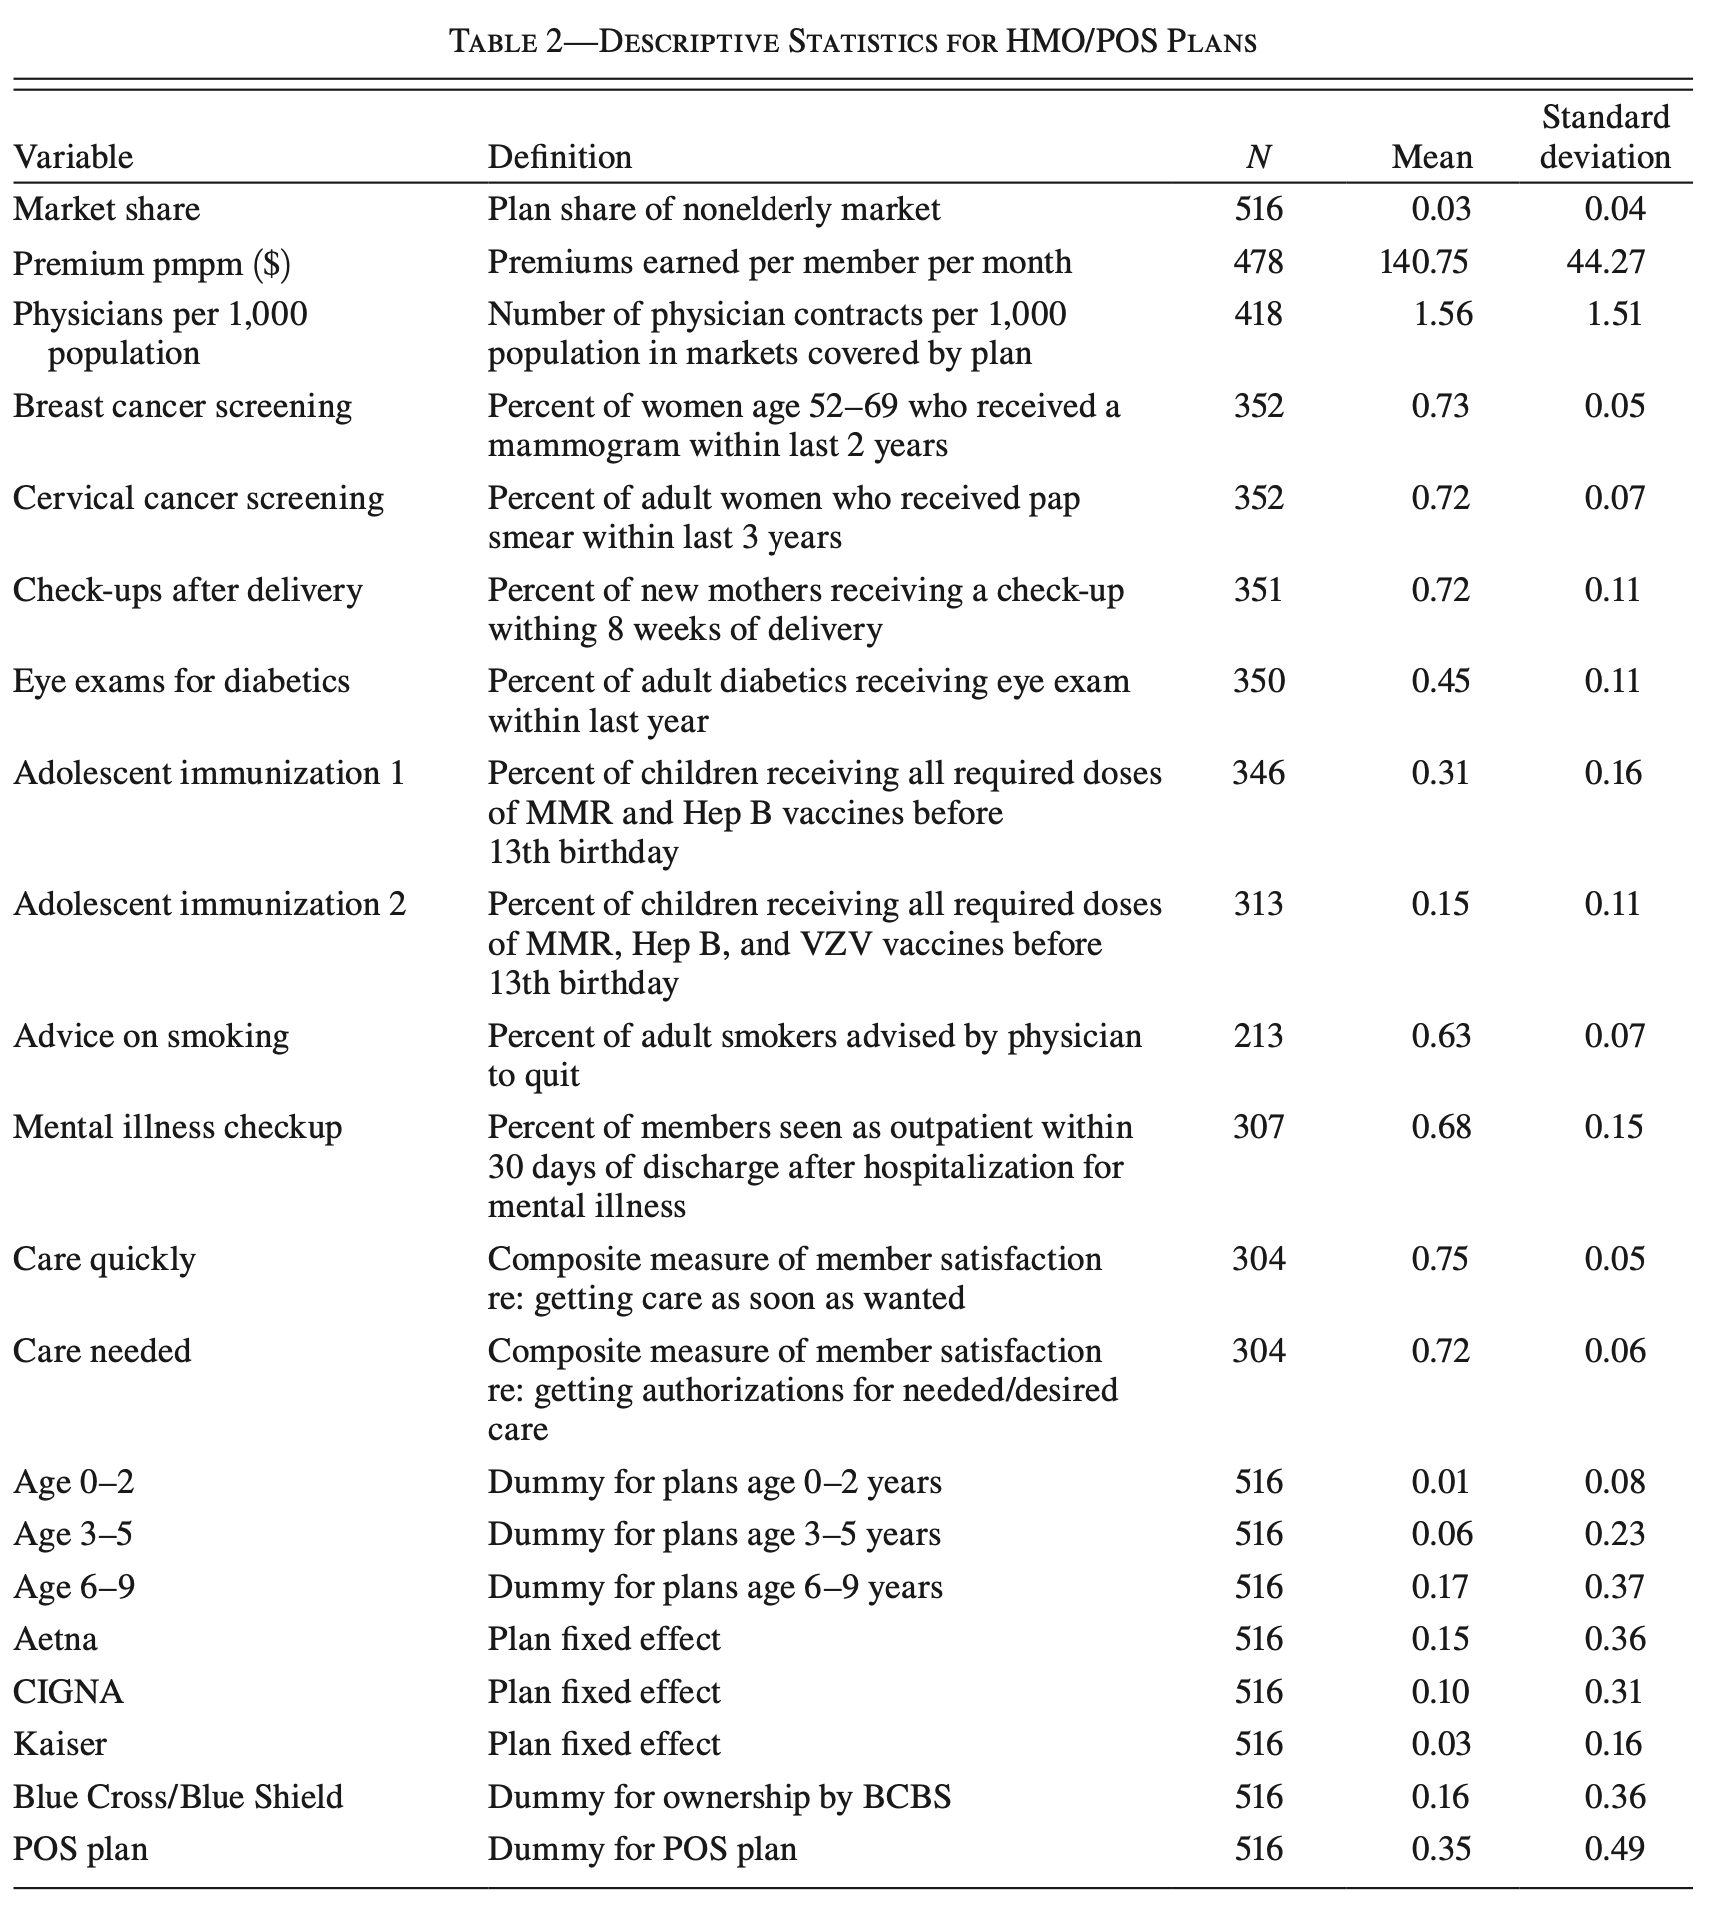
\includegraphics[height=7.5cm]{./resources/ho_table2.png}
\end{center}
\end{frame}

\begin{frame}{Network Choices}
\begin{itemize}
\item If all hospitals contract with all plans -- we can't tell who has bargaining power.\\
\end{itemize}
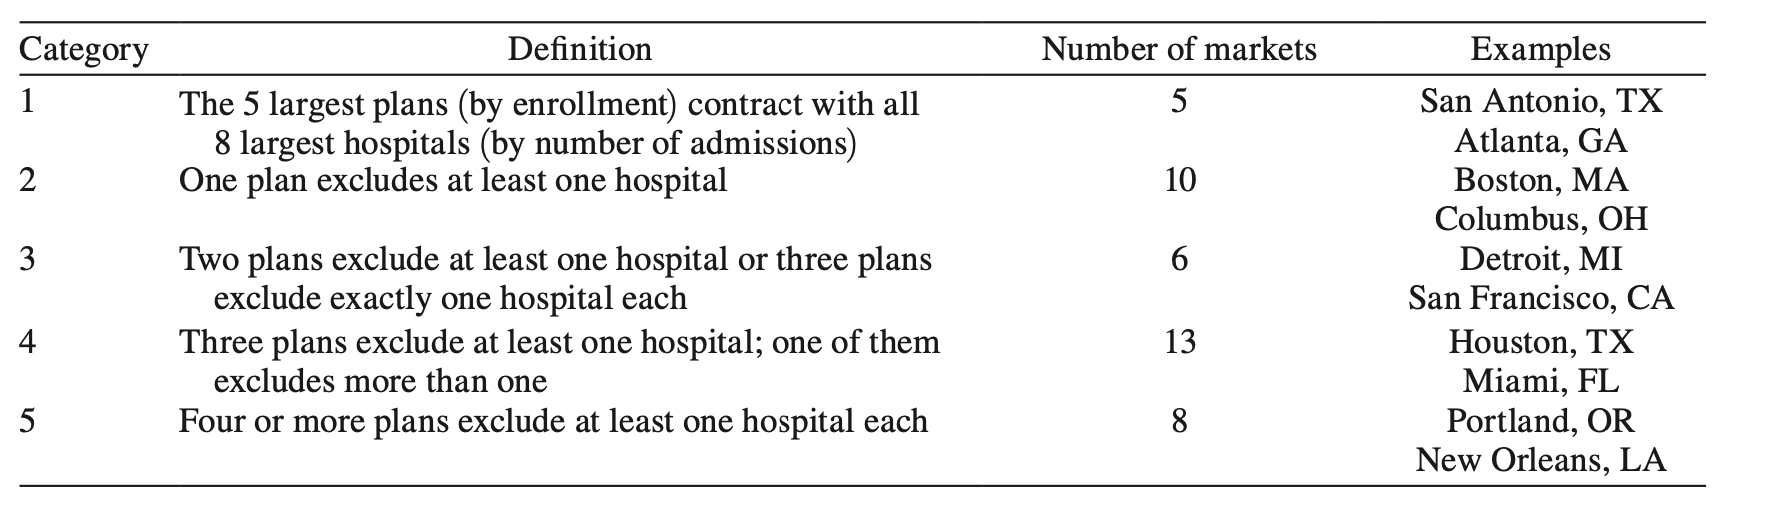
\includegraphics[height=4cm]{./resources/ho_fig1a.png}
\end{frame}



\begin{frame}{Network Choices}
\begin{center}
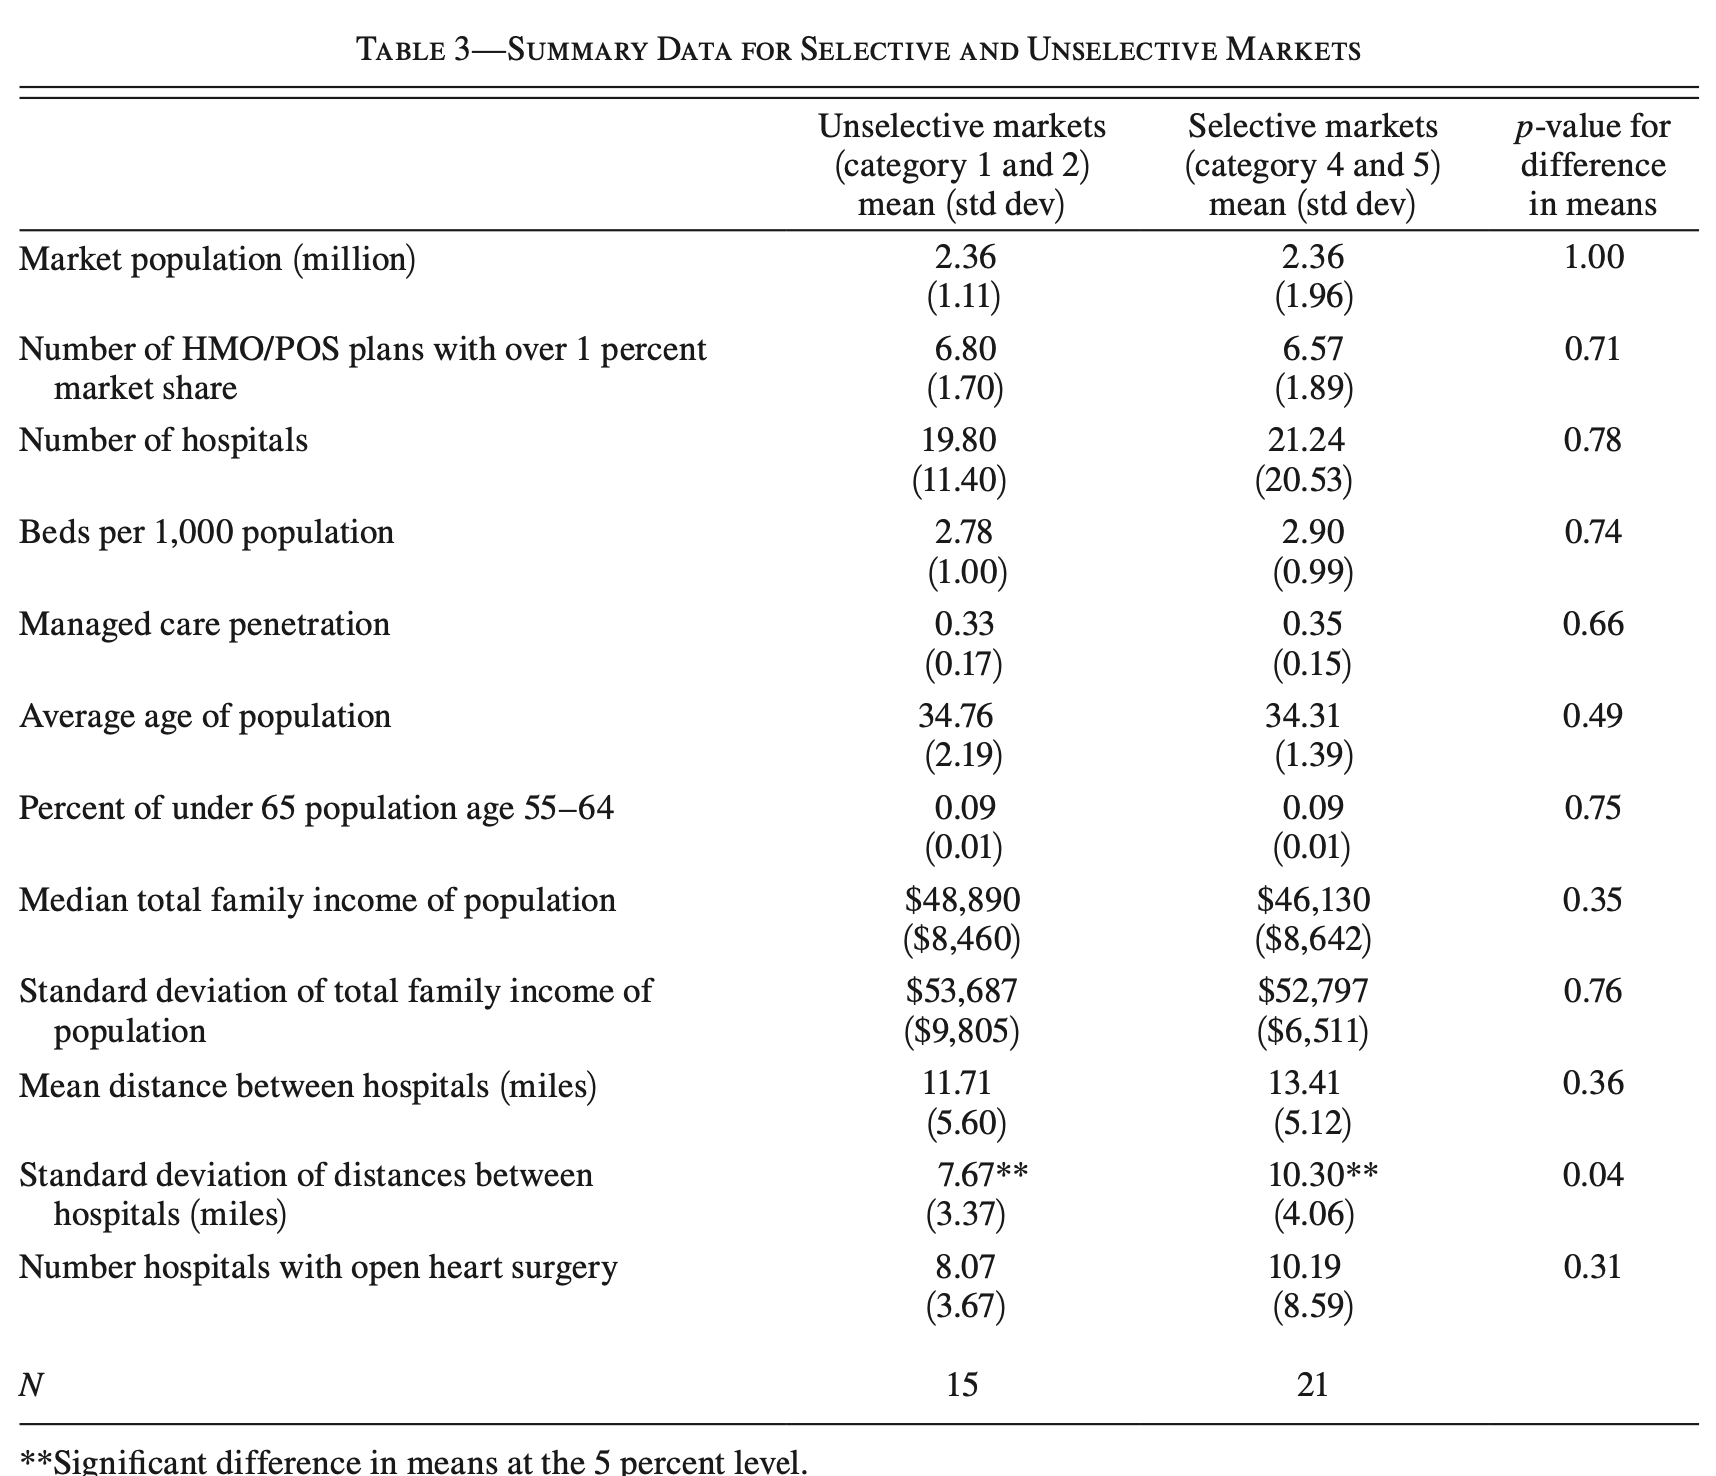
\includegraphics[height=7.5cm]{./resources/ho_table3.png}
\end{center}
\end{frame}

\begin{frame}{Hospital Demand}
Plain logit MLE (no random coefficients, no endogeneity)
\begin{itemize}
\item Similar to CDS (2003)
\item individual $i$, hospital $h$ and diagnosis $l$, and market $m$
\item Consumer characteristics $\nu_{i,l}$ (diagnosis, location, etc.)
\item $[x_h,\eta_h]$ hospital characteristics (obs, unobs)
\begin{align*}
u_{i, h, l}&=\eta_{h}+x_{h} \alpha+x_{h} v_{i, l} \beta+\varepsilon_{i, h, l} \\
E U_{i, j, m}&=\sum_{l} p_{i, l} \log \left(\sum_{h \in H j} \exp \left(\eta_{h}+x_{h} \hat{\alpha}+x_{h} v_{i, l} \hat{\beta}\right)\right)
\end{align*}
\item $p_{i,l}$ is ex-ante probability that consumer $i$ receives diagnosis $l$.
\end{itemize}
\end{frame}

\begin{frame}{Hospital Demand Results}
\begin{center}
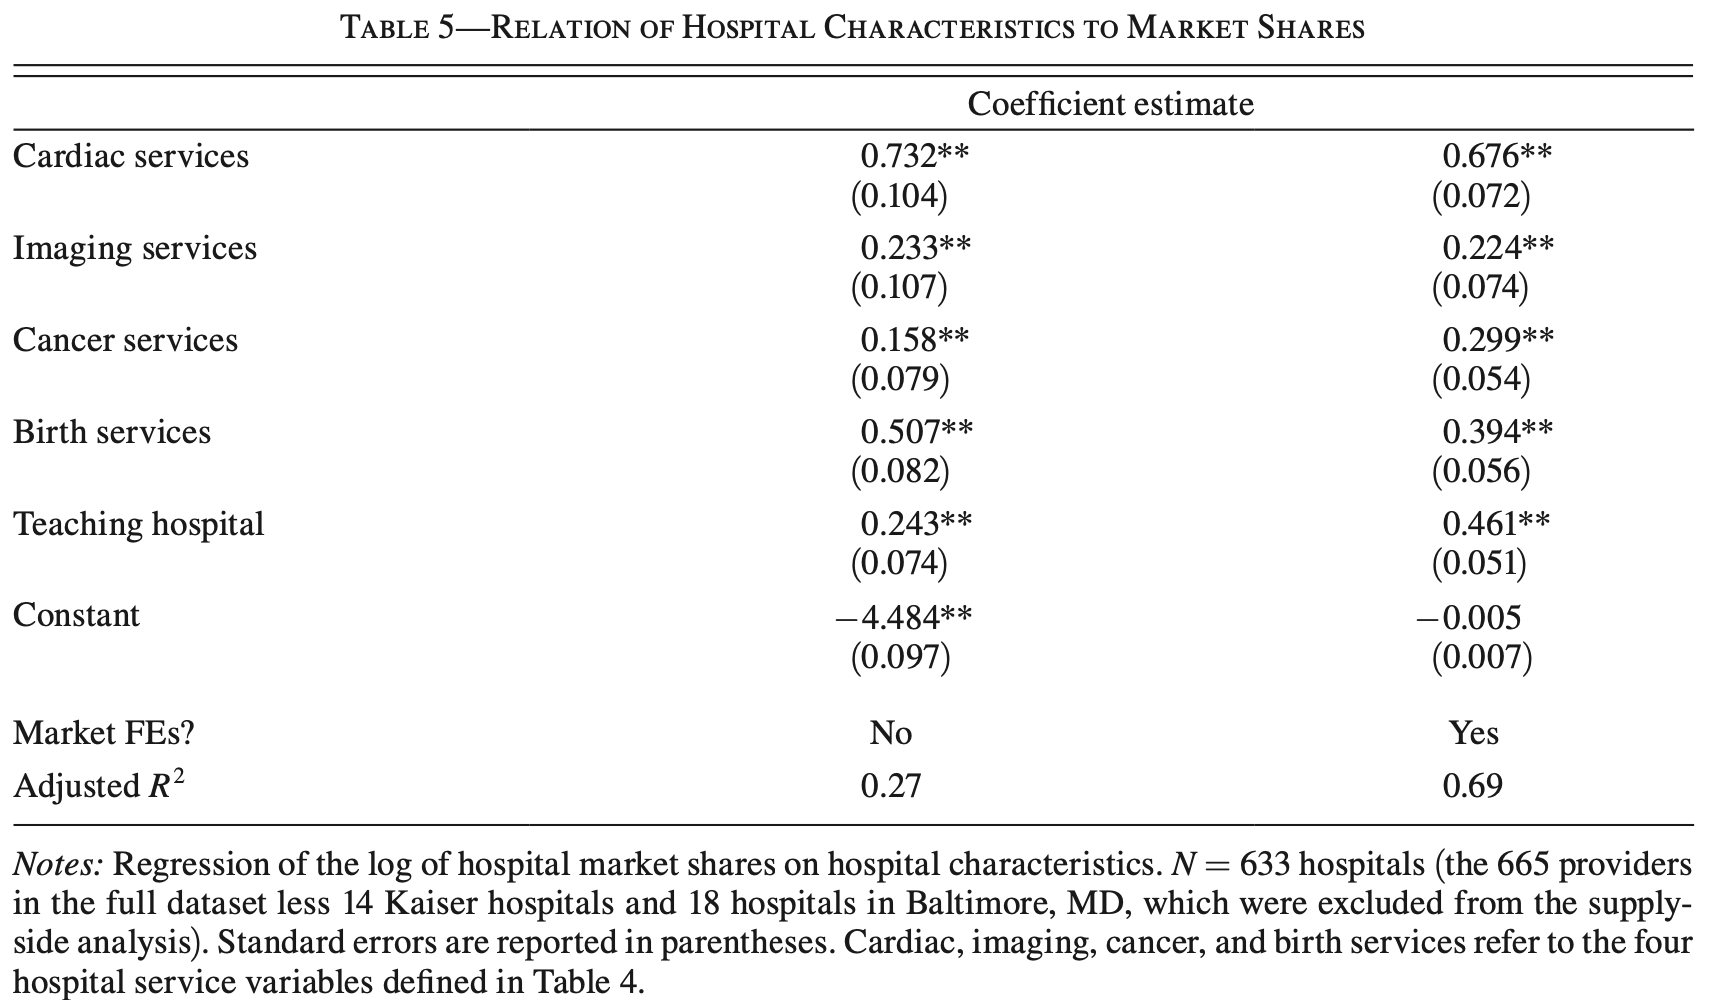
\includegraphics[height=7.5cm]{./resources/ho_table5.png}
\end{center}
\end{frame}

\begin{frame}{Plan Demand}
Take estimated $EU_{ijm}$ and include as a regressor in another logit for plan choice:
\begin{align*}
\tilde{u}_{i, j, m}=\xi_{j, m}+z_{j, m} \lambda+\gamma_{1} E U_{i, j, m}+\gamma_{2} \frac{ prem_{j, m}}{y_{i}}+\omega_{i, j, m}
\end{align*}
\begin{itemize}
\item $\xi_{jm}$ is unobserved plan quality (BLP type error)
\item $z_{jm}$ includes premium size of network, plan age, and clinical quality variables, consumer reported availability and speed scores.
\item Two outside goods: Idemnity (nonmanaged care: High), and Uninsured (Low)
\item Excluded IV: average hourly hospital wage, average weekly nurse wage across markets where plan is active. [Why?]
\end{itemize}
\end{frame}

\begin{frame}{Plan Demand Results}
\begin{center}
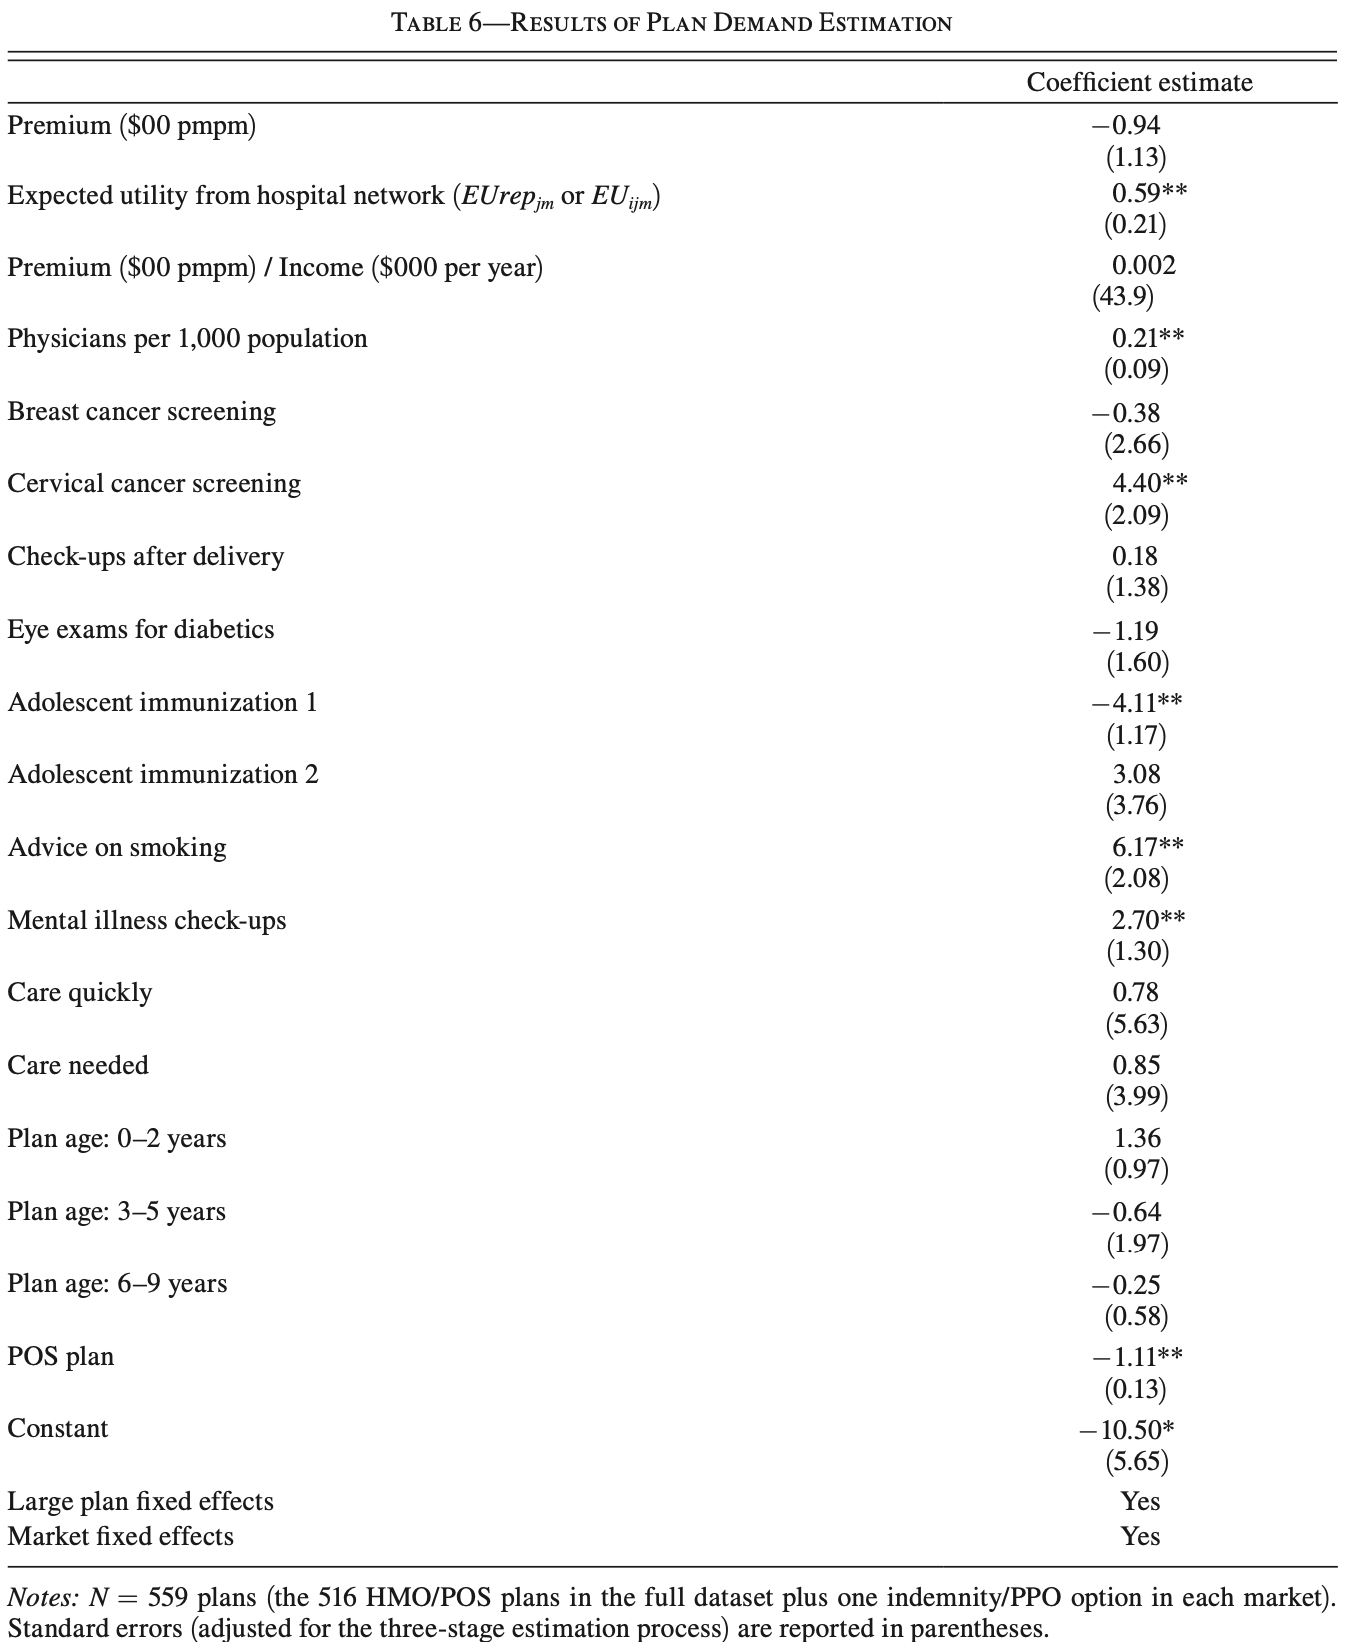
\includegraphics[height=7.5cm]{./resources/ho_table6.png}
\end{center}
\end{frame}

\begin{frame}{Producer Surplus for Network}
Surplus generated by plan $j$ in market $m$ with network $H_j$ is:
\begin{align*}
S_{j, m}\left(H_{j}, H_{-j}\right)=\sum_{i}\left(n_{i} s_{i, j, m}\left(H_{j}, H_{-j}\right)\left[prem_{j, m}-p_{i} \sum_{h \in H j} s_{i, h}\left(H_{j}\right)  cost_{h}\right]\right)
\end{align*}
\begin{itemize}
\item $n_i$ population per (ZCTA, age, gender) bin
\item $p_i$ admission probability of type $i$ individual
\item Plan $j$ offers network $H_j$ and rivals networks given by $H_{-j}$
 \item Prices and share (and costs) endogenously adjust. (Random re-allocation of patients at capacity constrained hospitals).
\end{itemize}
\end{frame}

\begin{frame}{Supply Intuition}
Why do not all hospitals reach agreement with all plans?
\begin{itemize}
\item Dropping plan $j$ from network changes both hospital demand and plan demand.
 \item Star Hospitals benefit from selecting contracting (consumers have high WTP)
 \item Hospital may be capacity constrained without contracting with all insurers (capacity may be endogenous)
 \item A large single system may be very attractive to consumers and induce consumers to switch (e.g. Harvard Pilgrim problem).
 \end{itemize}
\end{frame}


\begin{frame}{Producer Surplus for Network}
Profit is surplus generated $S_{jm}$ for network $H_j$ less cost:
\begin{align*}
\pi_{j, m}^{P}\left(H_{j}, \mathcal{H}_{-j}, \mathcal{X}, \theta\right)&=S_{j, m}\left(H_{j}, \mathcal{H}_{-j}\right)-c_{j, m}^{H O S P}\left(H_{j}, \mathcal{H}_{-j}, \mathcal{X}, \theta\right)-c_{j, m}^{N O N H O S P}\left(H_{j}, \mathcal{H}_{-j}, \mathcal{X}, \boldsymbol{\theta}\right) \\
\pi_{j, m}^{P, o}\left(H_{j}, \mathcal{H}_{-j}, \mathcal{X}^{o}, \theta\right)&=\pi_{j, m}^{P}\left(H_{j}, \mathcal{H}_{-j}, \mathcal{X}, \boldsymbol{\theta}\right)+u_{j, H}
\end{align*}
\begin{itemize}
\item First (eq) econometrician; second (eq) plan beliefs
\item Script variables are unobserved when plan makes contracting choice
\item Adds econometric error $u_{j,H_j}$ (measurement error) (Cost data is average not per patient)
\end{itemize}
Predicted profits from choosing $H_j$ can be written
\begin{align*}
E\left(\pi_{j, m}^{P}\left(H_{j}, \mathcal{H}_{-j}, \mathcal{X}, \theta\right) | I_{j, m}\right)=\pi_{j, m}^{P}\left(H_{j}, \mathcal{H}_{-j}, \mathcal{X}, \theta\right)-\varphi_{j, H_{j}}
\end{align*}
\end{frame}

\begin{frame}{Methodological Innovation}
\begin{itemize}
\item Plan $j$'s expected profits from network $H_j$ must exceed its expected profits from alternative network where it drops/adds hospital $h$ holding all else fixed
\item This represents \alert{necessary} but \alert{not sufficient} conditions for equilibrium.
\begin{align*}
E\left(\pi_{j, m}^{P}\left(H_{j}, \mathcal{H}_{-j}, \mathcal{X}, \boldsymbol{\theta}\right) | I_{j m}\right) \geq E\left(\pi_{j, m}^{P}\left(H_{j}^{h}, \mathcal{H}_{-j}, \mathcal{X}, \boldsymbol{\theta}\right) | I_{j, m}\right)
\end{align*}
Combine with both error terms:
\begin{align*}
\small
\pi_{j, m}^{P, o}\left(H_{j}, \mathcal{H}_{-j}, \mathcal{X}^{o}, \theta\right)-\pi_{j, m}^{P, o}\left(H_{j}^{h}, \mathcal{H}_{-j}, \mathcal{X}^{o}, \theta\right)\\
-\left(u_{j, H_{j}}-u_{j, H_{j}^{h}}\right)-\left(\varphi_{j, H_{j}}-\varphi_{j, H_{j}^{h}}\right) \geq 0
\end{align*}
Second term has expectation zero.
\end{itemize}
\end{frame}

\begin{frame}{Methodological Innovation}
\begin{itemize}
\item Resulting estimator combines \alert{moment equalities }$E[\xi_{jt}' z_{jt}]=0$ with \alert{moment inequalities}
\begin{align*}
\frac{1}{M} \sum_{m} \frac{\sqrt{n_{m}}}{n_{m}} \sum_{j=1}^{n_{m}}\left[\left(\pi_{j, m}^{P, o}\left(H_{j}, \mathcal{H}_{-j}, \mathcal{X}^{o}, \boldsymbol{\theta}\right)-\left(\pi_{j, m}^{P, o}\left(H_{j}^{h}, \mathcal{H}_{-j}, \mathcal{X}^{o}, \boldsymbol{\theta}\right)\right) \otimes g\left(z_{j, m}\right)\right] \geq 0\right.
\end{align*}
\item Penalize violations of moment equalities in both directions
\item Penalize violations of moment inequalities in only one direction.
\item Parameters may be \alert{set} rather than \alert{point identified}
\item Prof. Dickstein will talk more about estimation/inference.
\end{itemize}
\end{frame}



\begin{frame}{Full Results}
\begin{center}
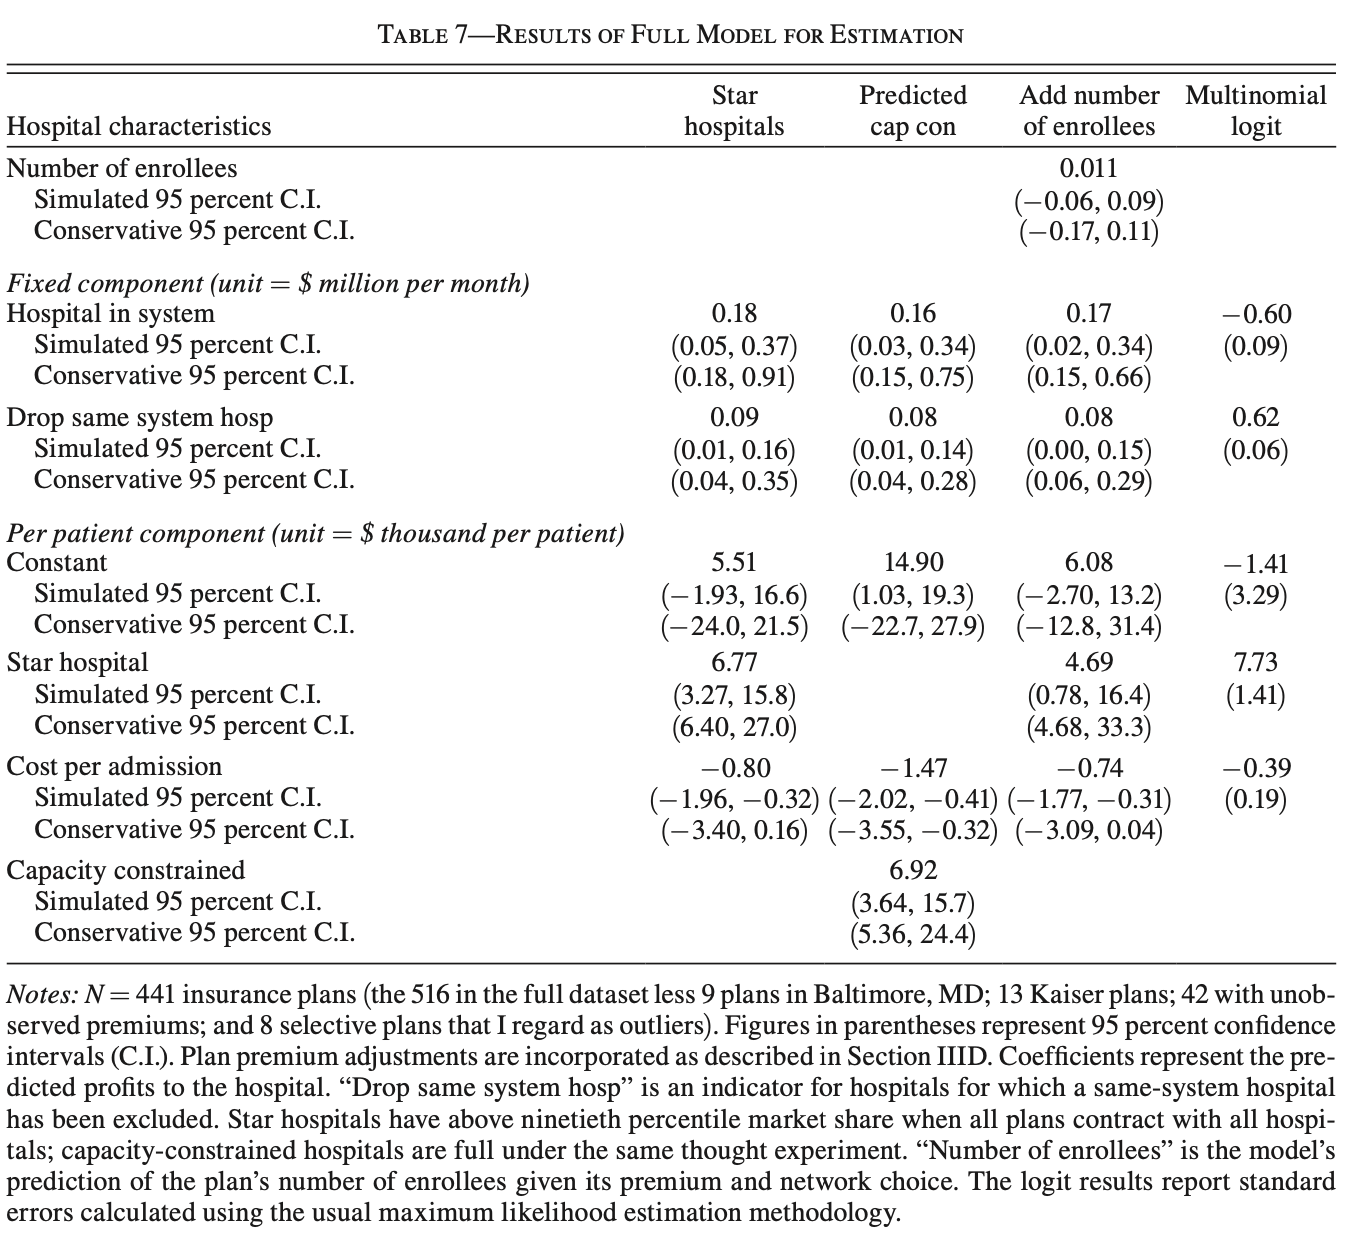
\includegraphics[height=7.5cm]{./resources/ho_table7.png}
\end{center}
\end{frame}

\begin{frame}{Full Results}
\begin{center}
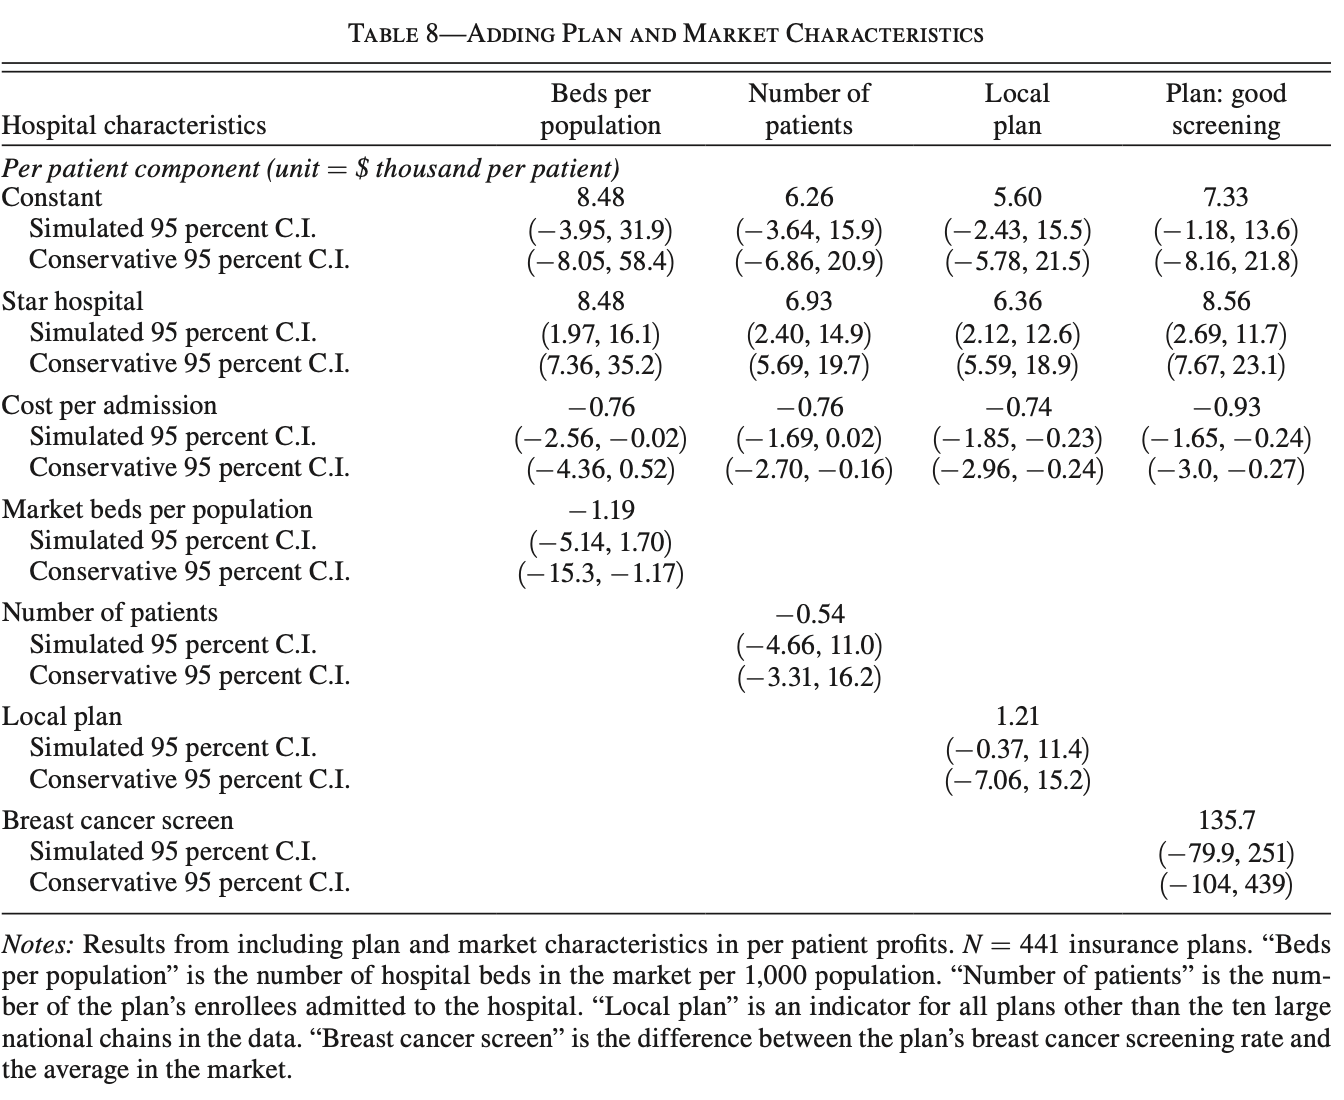
\includegraphics[height=7.5cm]{./resources/ho_table8.png}
\end{center}
\end{frame}

\begin{frame}{Full Results}
\begin{center}
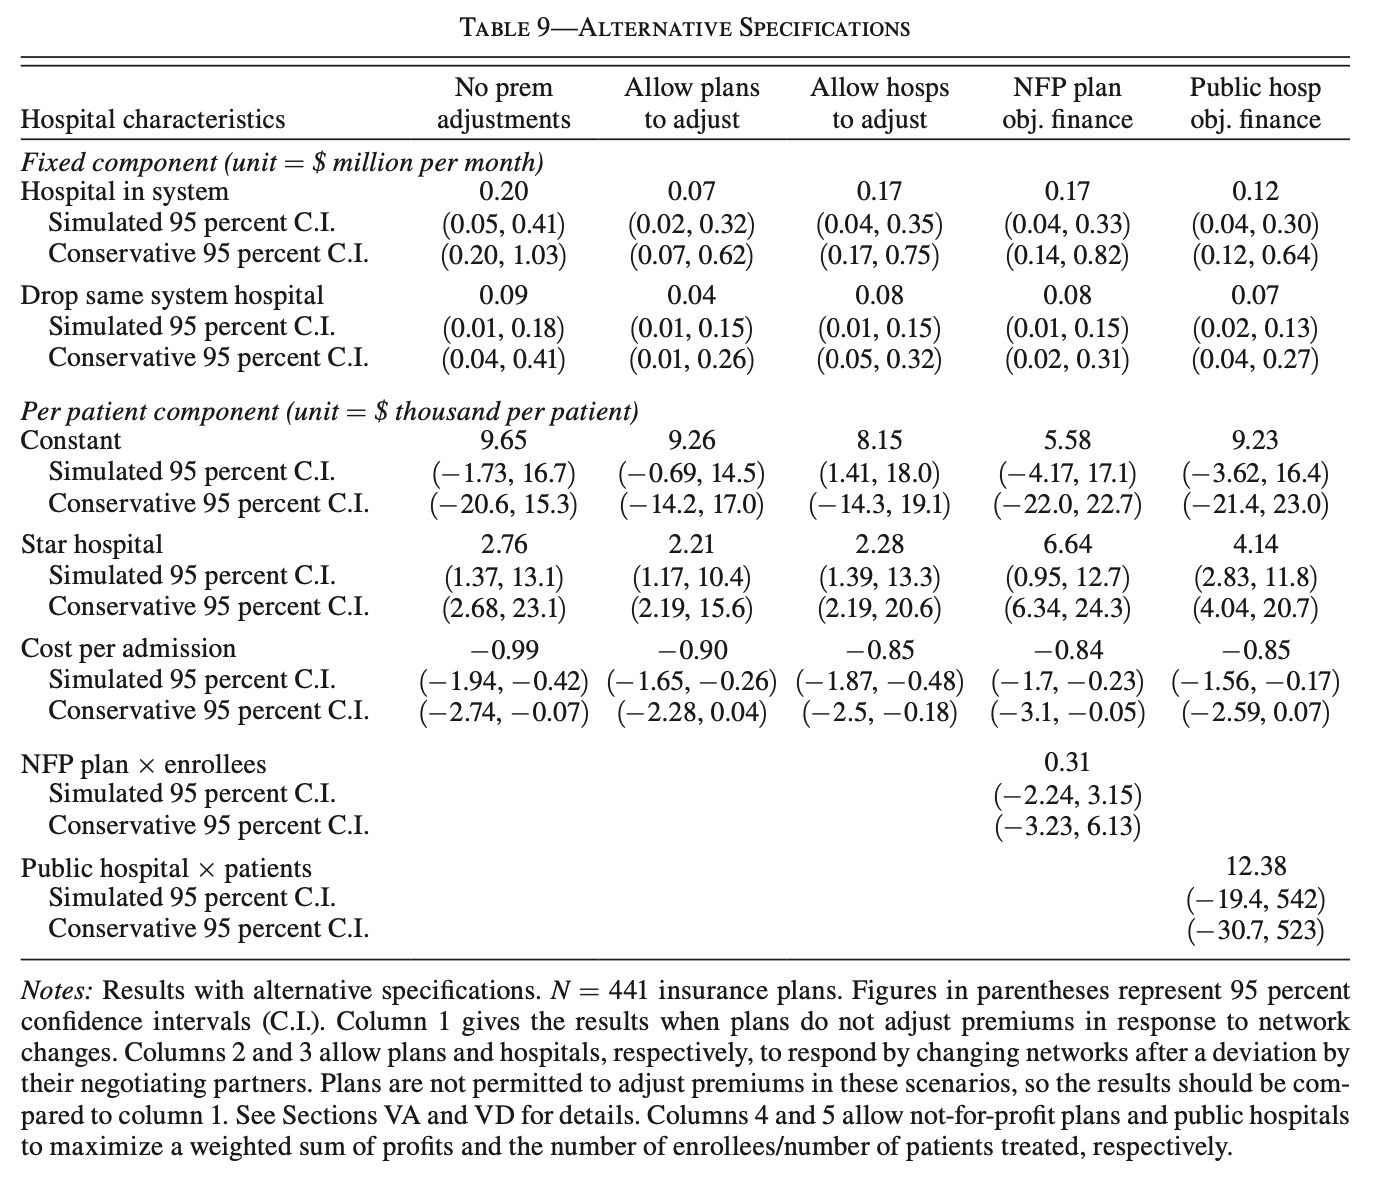
\includegraphics[height=7.5cm]{./resources/ho_table9.png}
\end{center}
\end{frame}
\begin{frame}{Full Results}
\begin{center}
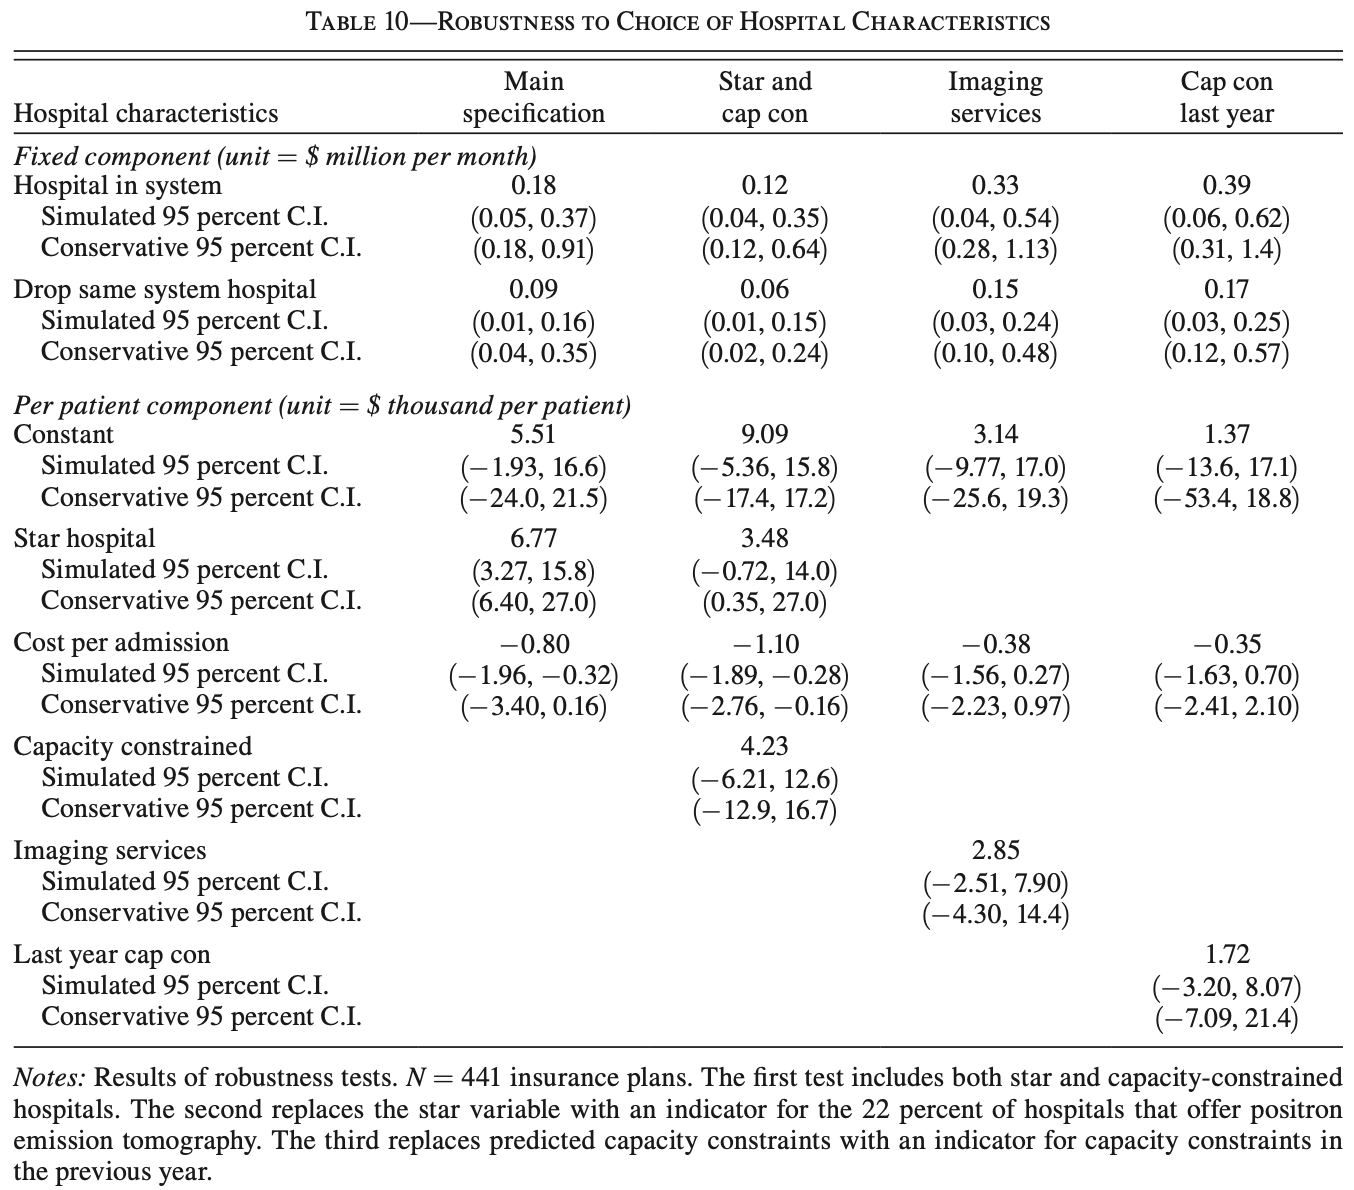
\includegraphics[height=7.5cm]{./resources/ho_table10.png}
\end{center}
\end{frame}

\begin{frame}{Recap}
\begin{itemize}
\item Hospitals bear about 80\% of their own costs. Why?
\item Providers have incentive to merge.
\item Becoming capacity constrained looks attractive.
\item Choice/access is valuable to consumers even for seldom chosen ``star'' hospitals that are far away.
\end{itemize}

\end{frame}

\end{document}













































